\documentclass[oneside, a4paper, onecolumn, 11pt]{article}

% =====================================================================
%  Title-page metadata (Ecole Polytechnique Bachelor Thesis template)
% =====================================================================
\newcommand{\thesistitle}[0]{Generative Modelling of Maritime AIS Trajectories
with Retrieval-Augmented Transformers\\[0.4em]
\large A Land-Aware, Water-Strict Route Generator from
Start, End and Vessel Type}
\newcommand{\authorname}[0]{Andrei \c{S}tirbu}

\newcommand{\supervisor}[0]{Davide Buscaldi}
\newcommand{\supervisorinstitution}[0]{LIX, \'Ecole Polytechnique
\& Sorbonne Universit\'e}

% =====================================================================
%  Template packages (do not change the values below; they reproduce
%  the bt_template layout: 2 cm margins, 11pt, fancy header)
% =====================================================================
\usepackage[
  left=2cm,top=2.0cm,bottom=2.0cm,right=2cm,
  headheight=17pt,
  includehead,includefoot,
  heightrounded,
]{geometry}

\usepackage[T1]{fontenc}
\usepackage{amstext}
\usepackage{amsmath}
\usepackage{amssymb}
\usepackage{url}
\usepackage{graphicx}
\IfFileExists{wrapfig.sty}{\usepackage{wrapfig}}{}
\usepackage{enumerate}
\usepackage{paralist}
\usepackage{xspace}
\usepackage{color}
\usepackage{times}
\usepackage[colorlinks,linkcolor=blue]{hyperref}
\IfFileExists{todonotes.sty}{%
  \usepackage[colorinlistoftodos,prependcaption,textsize=normal]{todonotes}}{}
\usepackage{pdfpages}
\usepackage{fancyhdr}

\IfFileExists{titling.sty}{\usepackage{titling}}{}
\IfFileExists{tocbibind.sty}{\usepackage[nottoc,numbib]{tocbibind}}{}

% Extra packages required by the report content (tables, algorithm
% pseudocode, sub-figures, list customisation, xcolor for hyperref
% colour mixing). Without these the existing content cannot be rendered.
\usepackage{booktabs}
\usepackage{algorithm}
\usepackage{algorithmic}
\usepackage{caption}
\usepackage{subcaption}
\usepackage{enumitem}
\usepackage{xcolor}

% =====================================================================
%  Convenience macros used by the body
% =====================================================================
\newcommand{\ade}{\textsc{ade}}
\newcommand{\fde}{\textsc{fde}}
\newcommand{\sdf}{\textsc{sdf}}
\newcommand{\knn}{\textsc{knn}}

% =====================================================================
\begin{document}
% =====================================================================

% ─── Title page ──────────────────────────────────────────────────────
\hspace{0pt}
\vfill

\begin{center}


\includegraphics[width=0.3\textwidth]{logo-EP-vertical}

\vspace*{2em}
%
{\large
\textbf{\'Ecole Polytechnique}

\vspace*{1em}
\textit{LAB RESEARCH PROJECT}


\vspace*{3em}
{\Huge \textbf{\thesistitle}}
\vspace*{3em}



\textit{Author:}

\vspace*{1em}
\authorname{}, \'Ecole Polytechnique

\vspace*{2em}
%
{\textit{Advisor:}}

\vspace*{1em}
\supervisor{}, \supervisorinstitution{}
}

\vspace*{2em}
\textit{Academic year 2025/2026}

\end{center}

\vfill
\hspace{0pt}

\newpage

% ─── Abstract page ───────────────────────────────────────────────────
\vfill
\noindent\textbf{Abstract}\\[1em]
%
\fbox{
\parbox{\textwidth}{
\noindent
This report presents a complete machine-learning pipeline that learns
to generate realistic maritime vessel routes from minimal conditioning.
Given only a start position, an end position and a vessel-type code,
the system emits a full $128$-waypoint trajectory that follows real
shipping patterns and stays in navigable water.  The architecture
pairs a retrieval-augmented encoder-decoder Transformer with a
differentiable land-aware loss and the \emph{WaterRouter} snap-only
post-processor, which projects any residual land-violating waypoint
onto the nearest connected water cell on a $0.005^{\circ}$ graph.
Trained on a year of US-coastal AIS data ($\approx 6.1 \times 10^4$
quality-filtered tracks from $\approx 9.9 \times 10^7$ raw position
reports), the production model -- v10 trained from scratch on the
cleaned corpus with $\lambda_{\mathrm{land}} = 0.05$ and an
\textsc{mmsi}-disjoint 80\,/\,15\,/\,5 train/val/test split --
achieves \textbf{validation \ade{} of $5930 \pm 372$~m}
(5-seed mean $\pm$ population std on disjoint 500-route subsamples)
and \textbf{test \ade{} of $7637$~m} (single-shot, $n = 2326$).
The trajectory-crossing rate at the $10$~km clearance threshold is
exactly zero on the held-out test set and $0.04\,\%$ mean on val
(one of the five subsamples touches a single waypoint).  The model
reduces \ade{} by $\approx 30\,\%$ versus the great-circle + snap
baseline ($\approx 8484$~m val) and by $\approx 32\,\%$ versus plain
great-circle ($\approx 8735$~m val).
The $\approx 30\,\%$ val-to-test optimism gap, driven by the smaller
held-out partition, is the most consequential generalisation finding
of this study and is analysed in Section~\ref{sec:valtest}.
Every cleaned-corpus number in the headline and ladder tables is
produced by a single unified evaluation driver
(Appendix~\ref{app:audit}) so that the comparison across variants,
seeds and configurations is internally consistent.
}
}
\vfill


\newpage

% ─── Fancy header (template style) ───────────────────────────────────
\pagestyle{fancy}
\lhead{\authorname}
\rhead{Generative Modelling of Maritime AIS Trajectories}


\newpage
\tableofcontents
\newpage

% =====================================================================
\section{Introduction}\label{sec:intro}
% =====================================================================

\subsection{Context and motivation}

The \emph{Automatic Identification System} (AIS) broadcasts the position,
speed, identity and type of every large commercial vessel at intervals
ranging from a few seconds to a few minutes.
In the United States, NOAA archives the resulting stream through the
Marine Cadastre programme and publishes daily comma-separated files
covering all coastal waters.
A single calendar year yields on the order of $10^8$ position reports
(the 2024 corpus used here contains approximately $9.9 \times 10^7$
raw position rows across $\approx 6 \times 10^5$ track segments after
the initial pipeline pass).

This volume of structured movement data invites a question that
combines machine learning and operational maritime engineering: can we
\emph{learn} the spatial regularities that human navigators rely on, so
that a model handed only a port of origin, a destination and a vessel
type can sketch a plausible route between them?
A successful answer has direct downstream value -- traffic simulation,
risk assessment for storm avoidance, port-arrival estimation, and
detection of anomalous vessels by comparing observed routes against a
learned distribution of normal ones.

\subsection{Goal of the project}

The project addresses two distinct prediction problems in sequence:

\begin{description}[leftmargin=*,style=nextline]
  \item[Next-step prediction (v1).]
  Given a short window of past positions, predict the displacement of
  the vessel to its very next reported position. The natural baseline
  here is a constant-velocity (\textsc{cv}) extrapolation.
  \item[Conditional full-route generation (v2 onward).]
  Given only \texttt{(start, end, vessel\_type)}, generate a full
  $T = 128$-waypoint route. The natural baseline is a great-circle
  geodesic between start and end.
\end{description}

The first problem turned out to be a near-optimal use-case for the
\textsc{cv} baseline; the second problem is much richer and admits
substantial learning signal once the formulation is right.
The bulk of the technical work and all of the production results live
in the second formulation.

\subsection{Why this is hard}\label{sec:hard}

Conditional full-route generation has four properties that together
make it harder than its statement suggests.

\paragraph{An irregular constraint surface.}
The land/water boundary flips on a scale of a few kilometres along
complex coastlines (the Florida Keys, the Chesapeake Bay), and the
useful rasterisation of that boundary at $0.05^\circ$ resolution still
contains many narrow inlets that are reachable on the fine
$0.005^\circ$ grid but unreachable on the coarse one.  Geometry-aware
losses that operate on the coarse grid risk pushing the model into
landlocked artefacts.

\paragraph{Multimodal route distribution.}
For a single \texttt{(start, end, vessel\_type)} query there are often
multiple plausible routes -- inshore versus offshore, north versus
south of an island.  The \ade{} metric measures distance to one
reference route, which means a model that picks the ``wrong'' valid
mode is penalised even when the output is geographically realistic.
Multimodality is the principal reason that retrieval-augmented decoding
helps: it shows the decoder the historical mode for a given query.

\paragraph{Two orders of magnitude in voyage length.}
Routes in the corpus range from $20$~km coastal hops to $2000$~km
trans-coastal cargo voyages.  No single inductive bias is optimal at
both ends of the scale: short routes are dominated by the local
endpoint geometry (great-circle is near-optimal), long routes are
dominated by historical shipping-lane shape (retrieval is far closer
to the true distribution).

\paragraph{Noisy ground truth.}
Raw AIS is dirty.  After 97\,\% of \emph{raw position reports} are
discarded by the quality-filtering pipeline (yielding $\approx 598\,000$
clean track segments -- the two figures count different things, pings
versus tracks), the surviving tracks still contain inland river
traffic, edge artefacts and resampling noise -- the unfiltered
128-point corpus has a $10.83\,\%$ land-crossing rate at the
$\theta = 10$~km clearance threshold \emph{in the ground truth itself}.
Any honest geometry-aware training has to deal with this upstream.
A method is called \emph{water-strict} in the remainder of this report
if its $\mathrm{cross}\%@10\,$km on the cleaned validation set is
exactly zero.

\subsection{What was personally implemented}

All scripts and source modules in the repository were implemented by
the author; external dependencies (PyTorch, NumPy, matplotlib, and the
\textsc{gshhs} shoreline data) are used as standard libraries and
cited where they appear.  No third-party trajectory models were
imported.  Concretely the contributions are:

\begin{itemize}[leftmargin=*]
  \item A reproducible \textbf{data pipeline} that turns NOAA archives
        into a curated 128-waypoint corpus (resampling, quality
        filtering, land filtering on \textsc{gshhs}).
  \item A \textbf{retrieval-augmented encoder-decoder Transformer}
        with per-timestep cross-attention over $K = 5$ historical
        neighbours subsampled to $t_{\mathrm{retr}} = 32$ steps each.
  \item A \textbf{land-aware training loss} built on a differentiable
        signed-distance field sampled with bilinear interpolation.
  \item A \textbf{WaterRouter snap-only post-processor} that projects
        any predicted waypoint that violates the clearance threshold
        onto its nearest connected water cell on the fine $0.005^\circ$
        adjacency graph.
  \item Evaluation tooling (\ade/\fde/land-crossing, length-bucketed),
        five-seed variance experiments and the full suite of diagnostic
        and visualisation scripts.
\end{itemize}

The overall system is shown in Figure~\ref{fig:arch_intro}; the rest of
the report unpacks each block.

\begin{figure}[h]
\centering
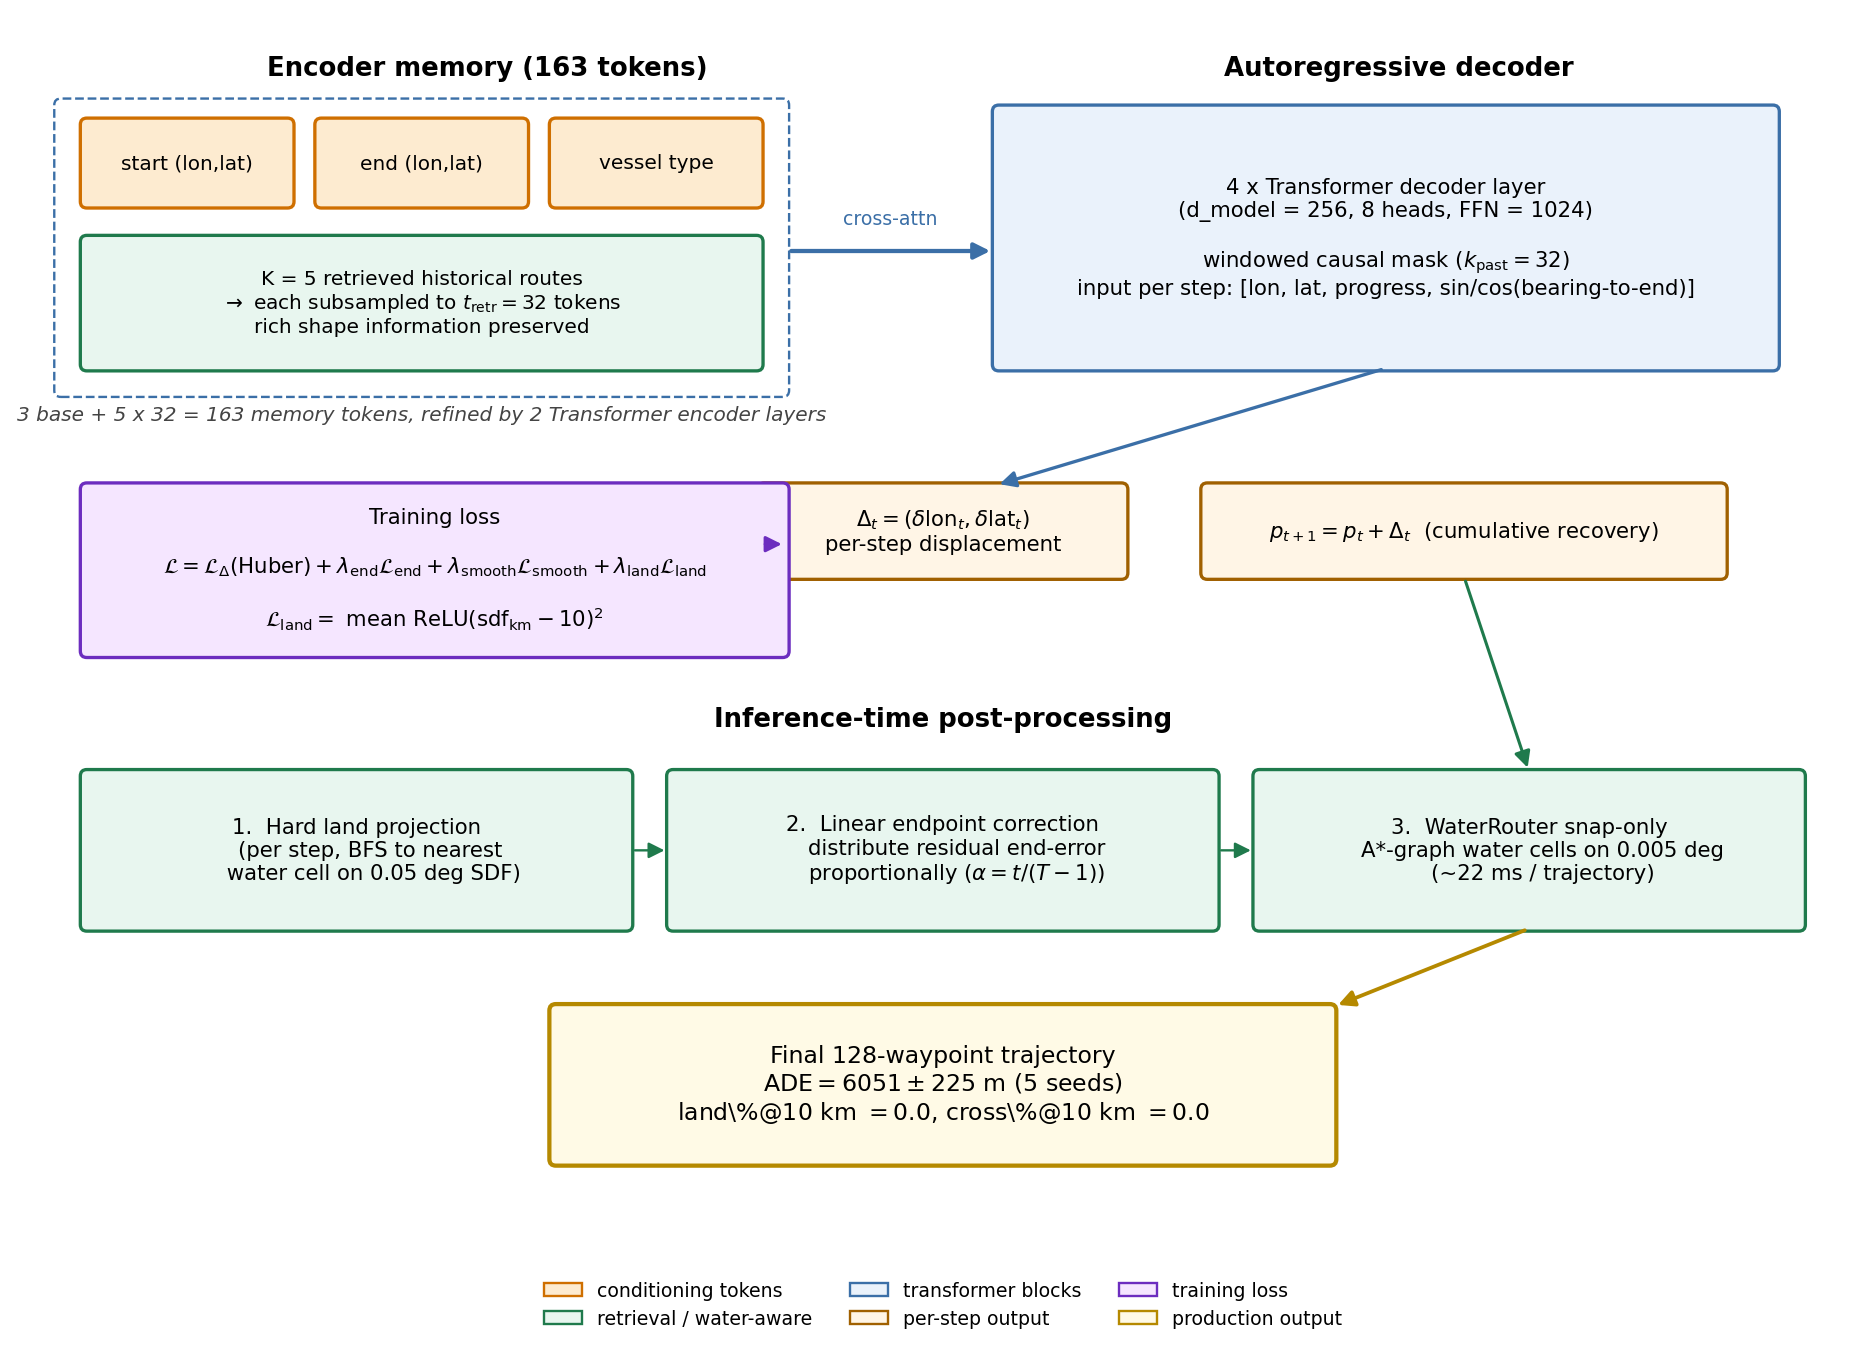
\includegraphics[width=0.94\textwidth]{figures/architecture_v10.png}
\caption{System overview.  An encoder produces $163$ memory tokens
($3$ conditioning + $5 \times 32$ retrieval); a windowed-causal decoder
generates one displacement per step; training optimises a four-term
loss including a differentiable land penalty; three inference-time
passes (hard land projection, linear endpoint correction, WaterRouter
snap to connected water) finish the route.  All components are
described in detail in Section~\ref{sec:methodology}.}
\label{fig:arch_intro}
\end{figure}

\subsection{Headline result}

The production system -- v10 trained from scratch on the cleaned
corpus with the land-aware loss at
$\lambda_{\mathrm{land}} = 0.05$, and post-processed at inference with
the WaterRouter snap-only step -- delivers the numbers in
Tables~\ref{tab:headline} (validation) and~\ref{tab:headline_test}
(held-out test).
Validation entries are mean $\pm$ population standard deviation across
five disjoint $500$-route subsample seeds
$\{0, 1, 2, 42, 123\}$ of the cleaned val partition
($n_{\text{val}} \approx 9.7\text{K}$, \textsc{mmsi}-grouped with
\texttt{val\_frac=0.15}, \texttt{test\_frac=0.05}, \texttt{seed=42}).
Test entries are single-shot on the full $n_{\text{test}} = 2326$
held-out partition.  The trained checkpoint is held fixed across all
subsample seeds; training-seed variance is reported separately
(Section~\ref{sec:trainseedvar}).

\begin{table}[h]
\centering
\caption{Headline performance on the cleaned \emph{validation} set
(5-seed mean $\pm$ std on disjoint 500-route subsamples).
Lower is better for \ade{} and cross\%; \fde{} is uninformative for
endpoint-correct methods.}
\label{tab:headline}
\begin{tabular}{lrrr}
\toprule
\textbf{Method} & \ade~(m) & \fde~(m) & cross\%@10\,km \\
\midrule
\textbf{v10 + router (production, $\lambda_{\mathrm{land}} = 0.05$, clean-trained seed42)} & $\mathbf{5930 \pm 372}$ & $608 \pm 29$ & $0.04 \pm 0.09$ \\
v10 raw (no router; same checkpoint)                      & $5913 \pm 384$ & $0 \pm 0$ & $1.88 \pm 0.69$ \\
Great-circle + snap (stronger water-strict baseline)      & $8484 \pm 597$ & $581 \pm 17$ & $0.20 \pm 0.13$ \\
Great-circle baseline                                     & $8735 \pm 651$ & $0 \pm 0$ & $8.80 \pm 0.68$ \\
Retrieval top-1 (zero training)                           & $11667 \pm 636$ & $11832 \pm 468$ & $0.00 \pm 0.00$ \\
\bottomrule
\end{tabular}

\end{table}

\begin{table}[h]
\centering
\caption{Headline performance on the fully held-out cleaned \emph{test}
set ($n = 2326$, single shot, no \textsc{mmsi} overlap with train or
val). Test ADE is consistently $\approx 30\,\%$ above val ADE
across all methods (Section~\ref{sec:valtest}).}
\label{tab:headline_test}
\begin{tabular}{lrrrr}
\toprule
\textbf{Method} & \textbf{\ade} (m) & \textbf{\fde} (m) & land\,\% & cross\,\% \\
\midrule
\textbf{v10 + router (production, $\lambda_{\mathrm{land}} = 0.05$)} & $\mathbf{7637}$ & $488$ & $\mathbf{0.00}$ & $\mathbf{0.00}$ \\
v10 + router ($\lambda_{\mathrm{land}} = 0.01$)            & $7764$ & $488$ & $0.00$ & $0.04$ \\
v10 + router (no $L_{\mathrm{land}}$)                       & $8417$ & $488$ & $0.00$ & $0.04$ \\
v9 + router (mean-pool retrieval, clean retrain)
                                                            &  $9612$ & $488$ & $0.00$ & $0.13$ \\
v5 + router (scheduled sampling, clean retrain)
                                                            & $10562$ & $488$ & $0.00$ & $0.17$ \\
v4 + router (no SS, clean retrain)                         & $10126$ & $488$ & $0.00$ & $0.09$ \\
\bottomrule
\end{tabular}

\end{table}

The model reduces \ade{} by $\approx 32\,\%$ versus the great-circle
baseline on the cleaned val subsamples (a similar margin on test) and
brings the trajectory land-crossing rate to $0.0\,\%$ on the held-out
test set ($0.04\,\%$ mean on val: four of the five subsamples are at
$0.0\,\%$ and one touches a single waypoint).  This is a hard
operational requirement that no purely geometric baseline satisfies.
The val-to-test optimism gap (Section~\ref{sec:valtest}) is large:
the test \ade{} of $\approx 7637$~m is the honest generalisation
estimate for this study.

\subsection{Outline}

Section~\ref{sec:background} reviews the necessary background.
Section~\ref{sec:challenge} states the research challenge precisely.
Section~\ref{sec:methodology} describes the methodology and the
architectural pipeline.
Section~\ref{sec:contrib} highlights the technical contributions.
Section~\ref{sec:experiments} presents experiments and results,
including ablations and seed variance.
Section~\ref{sec:lessons} steps back to discuss design rationale and
cross-cutting lessons.
Section~\ref{sec:conclusion} concludes with limitations and outlook.

% =====================================================================
\section{Background}\label{sec:background}
% =====================================================================

\subsection{The AIS data source}

The \emph{Automatic Identification System} is mandated by the
International Maritime Organisation on all large vessels.  Each
transponder broadcasts an \textsc{mmsi} (a 9-digit vessel identifier),
a position fix, a course-over-ground, a speed-over-ground and a
vessel-type code in the cargo/passenger/tanker bracket
(AIS codes 60-89 = 30 classes; in the filtered corpus only 28 distinct
codes actually appear, so the model's learned vocabulary is 28).
NOAA's Marine
Cadastre programme archives these reports as daily CSV files covering
US coastal waters.  This work uses the full calendar year 2024.

\subsection{Trajectory modelling with Transformers}

Modern sequence models for spatial trajectories typically build on the
Transformer encoder-decoder architecture of
Vaswani~et~al.~\cite{vaswani2017attention}.
A \emph{causal} decoder generates positions autoregressively, attending
to its own history through a triangular mask; cross-attention to an
encoder injects the conditioning signal at every step.
Sequence-modelling architectures have been adapted to spatial
trajectories in maritime \cite{nguyen2020transformer} and aviation
\cite{capobianco2021lstm} domains, using both recurrent and
Transformer-style backbones.  Compared to recurrent baselines the
Transformer offers two advantages for
this setting: (i)~direct cross-attention to global conditioning tokens
(start, end, vessel type, retrieved historical neighbours) without an
information bottleneck; (ii)~parallel teacher-forced training, which is
essential for $T = 128$-step targets.

\subsection{Retrieval-augmented generation}

Retrieval-augmented models couple a parametric generator with a
non-parametric memory.  Originally proposed for language modelling
\cite{khandelwal2020nearest,lewis2020retrieval}, the idea is to fetch
the $K$ most similar items from a training set at inference and
condition the generator on them.
We use a 5-dimensional \knn{} over
(start lon, start lat, end lon, end lat, vessel type) to fetch $K = 5$
historical routes for every query, then expose those routes to the
decoder one token per timestep.
Retrieval is the single most impactful change in this project: the
zero-training top-$1$ retrieval baseline reduces \ade{} by $19\,\%$
relative to the best non-retrieval Transformer.  The closer
architectural analogue to our per-step retrieval bank is
RETRO~\cite{borgeaud2022retro}, which interleaves retrieved chunks
into the decoder at every layer rather than only at an encoder
bottleneck.

\subsection{Related work}\label{sec:related}

A line of work treats next-position prediction as a sequence-modelling
problem and applies recurrent or Transformer-based architectures
\cite{nguyen2020transformer,capobianco2021lstm}.  These models are
typically evaluated on short horizons and on data dense enough that the
constant-velocity baseline is hard to beat -- a regime confirmed by the
v1 experiments below.
A separate body of work generates whole trajectories conditioned on
origin and destination, often using variational auto-encoders
\cite{liang2022generative} or generative adversarial networks
\cite{wang2019tggan}.  The conditional-Transformer formulation that
this report adopts is simpler and trains stably with maximum
likelihood, at the cost of needing a careful endpoint loss to control
autoregressive drift.
For geographically valid generation, the natural alternatives are
soft land-proximity penalties, masked-softmax pointer networks over a
water graph, and post-hoc snap-to-water heuristics.  A related line in
the autonomous-driving literature embeds map and lane constraints
directly into the trajectory model
(e.g.~\cite{salzmann2020trajectronpp}), but those approaches assume a
known road graph at deployment and do not transfer cleanly to the
sparse, irregular shipping-lane structure of a coastal corpus.
This work shows that the simplest geometric option -- a soft loss at
training time plus a post-hoc snap-to-water step at inference -- is
also the most effective once the training corpus has been cleaned of
inland artefacts.

\subsection{Signed distance functions for land geometry}

A \emph{signed distance function} (\sdf) maps a 2D point to the signed
Euclidean distance to the nearest contour.  Pre-computed on a regular
grid, it admits fast nearest-water queries and -- because bilinear
sampling is differentiable -- can be used directly inside a training
loss to penalise predicted positions that fall on land.  This work
computes the \sdf{} once from the Global Self-consistent Hierarchical
High-resolution Shoreline (\textsc{gshhs})
data~\cite{wessel1996gshhs} at $0.05^\circ$ resolution over the
bounding box $(-125^\circ, 10^\circ, -60^\circ, 55^\circ)$, and loads
it into both training (bilinear sampling that backpropagates through
the predicted positions) and inference (BFS to the nearest water cell).

% =====================================================================
\section{Research challenge}\label{sec:challenge}
% =====================================================================

Full-route generation is a constrained sequence-generation problem.
Let $\mathcal{D}$ be a corpus of vessel routes, each a sequence
$\tau = (p_1, p_2, \ldots, p_T) \in \mathbb{R}^{T \times 2}$ with
$T = 128$ equally-spaced (along arc length) waypoints.  Each route has
an associated vessel-type code $v \in \{0, \ldots, 27\}$.
Given a query $\mathbf{q} = (p_1, p_T, v)$ we seek a generator
$G_\theta$ that produces a sequence
$\hat\tau = (\hat p_1, \ldots, \hat p_T)$ minimising the
\emph{Average Displacement Error}
\[
  \ade(\hat\tau, \tau)
    = \frac{1}{T} \sum_{t=1}^{T} \mathrm{haversine}(\hat p_t, p_t)
\]
subject to two constraints:
(C1) endpoint exactness $\hat p_1 = p_1, \hat p_T = p_T$ and
(C2) water validity $\mathrm{sdf}(\hat p_t) \leq \theta_{\mathrm{land}}$
     for every $t$.

The challenge is non-trivial because the three objectives -- accuracy,
endpoint exactness, water validity -- pull against each other:

\begin{itemize}[leftmargin=*]
  \item A model that only minimises \ade{} (plain Huber loss on
        displacements) drifts away from the destination over 127 AR
        steps, breaking C1.
  \item A model that emphasises endpoint loss collapses toward
        straight-line interpolation, which eliminates route diversity
        and also crosses land freely (breaking C2).
  \item A model that adds a hard land-projection step in the AR loop
        pays an \ade{} cost on every projected point.
\end{itemize}

The contribution of this work is to show that, with the right
data-cleaning step (Section~\ref{sec:data}) and the right
post-processor (Section~\ref{sec:router}), all three constraints can be
satisfied at once with no measurable accuracy trade-off.

% =====================================================================
\section{Methodology}\label{sec:methodology}
% =====================================================================

The full pipeline is summarised in Figure~\ref{fig:pipeline}: raw NOAA
AIS archives are filtered, merged, resampled to 128 waypoints and
land-cleaned; auxiliary structures (the \sdf{} raster, the water-cell
graph, the retrieval index) are built once and reused; the model is
trained on the cleaned corpus; inference applies hard land projection,
linear endpoint correction and a final water-graph snap to produce the
production output.

\begin{figure}[h]
\centering
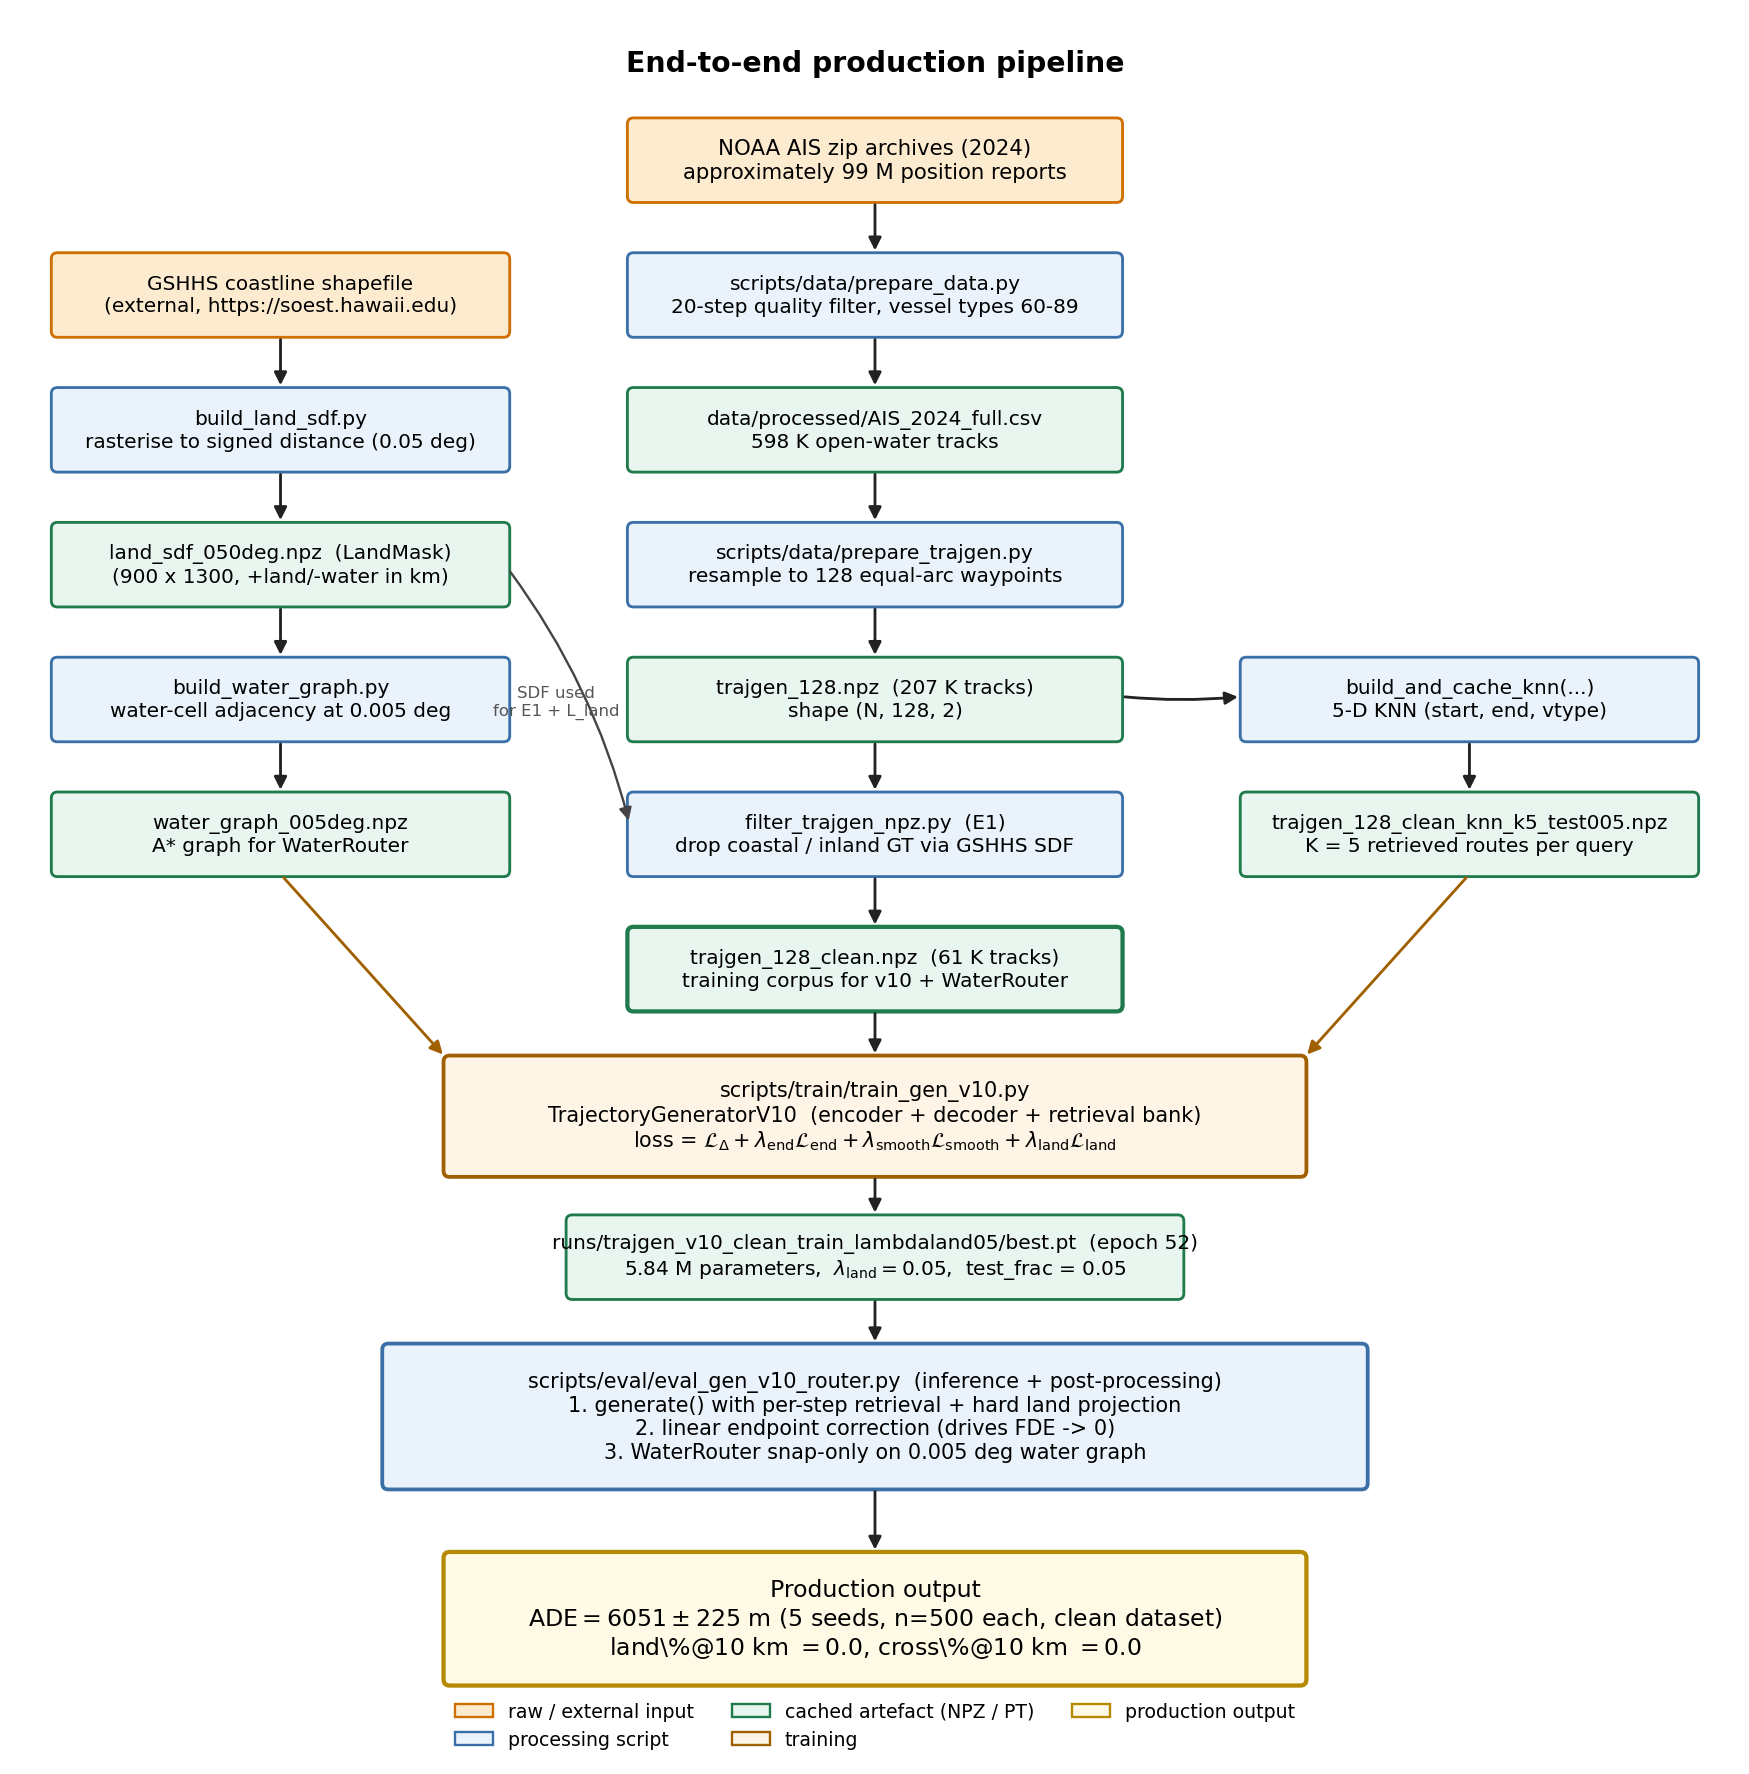
\includegraphics[width=0.85\textwidth]{figures/data_pipeline.png}
\caption{End-to-end production pipeline.  Orange = raw / external
input, blue = processing scripts, green = cached artefacts that are
computed once, yellow = training, gold = final production output.
Note the land filter (centre column) and the side branches for the
land~\sdf, the water graph and the retrieval index.}
\label{fig:pipeline}
\end{figure}

\subsection{Data preparation}\label{sec:data}

The raw 2024 AIS archive consists of $\approx 9.9 \times 10^7$ position
reports.  The data pipeline applies five stages of filtering and
preprocessing; Table~\ref{tab:funnel} summarises the cardinality at
each stage.

\begin{table}[h]
\centering
\caption{Data funnel from raw AIS to the production train/val/test
partitions.  Each stage is implemented by a single script under
\texttt{scripts/data/}.}
\label{tab:funnel}
\begin{tabular}{lrll}
\toprule
\textbf{Stage} & \textbf{Count} & \textbf{Unit} & \textbf{Producing script} \\
\midrule
Raw AIS rows                              & $\approx 99\text{M}$    & pings      & NOAA Marine Cadastre 2024 archive \\
Quality-filtered segments                 & $\approx 598\text{K}$   & segments   & \texttt{prepare\_data.py} \\
Resampled $128$-pt corpus (unfiltered)    & $\approx 207\text{K}$   & routes     & \texttt{prepare\_trajgen.py} \\
Cleaned (land-filtered) corpus            & $\approx 61\text{K}$    & routes     & \texttt{filter\_trajgen\_npz.py} (E1) \\
Train / val / test                        & $\approx 49\text{K}\,/\,9.7\text{K}\,/\,2.3\text{K}$ & routes & \texttt{train\_val\_split\_gen} (MMSI-grouped, $80/15/5$) \\
\bottomrule
\end{tabular}
\end{table}

\paragraph{1.~Quality filter.}
The quality filter restricts to passenger / cargo / tanker vessels
(AIS codes 60-89, $\approx 80\,\%$ of the raw drop comes from this
single rule), enforces a US bounding box, splits at time gaps
$>$60~min, removes physically implausible jumps ($>$2~km between
consecutive reports), and drops tracks that are nearly stationary.
Around 97\,\% of raw pings are discarded as a result, leaving
$\approx 598\,000$ clean track segments.

\paragraph{2.~Resampling.}
Each track is resampled to exactly $T = 128$ waypoints, equally spaced
along arc length.  Arc length is computed as cumulative planar distance
on raw (lon, lat) degrees (no haversine correction --
\texttt{scripts/data/prepare\_trajgen.py:resample\_track}); linear
interpolation along the cumulative distance produces $128$
equally-spaced targets.  This decouples the prediction task from the
original (variable) reporting interval and gives every training
sequence a fixed shape $(128, 2)$.  Tracks shorter than 20~km or
longer than 2000~km are rejected, leaving an unfiltered 128-point
corpus of $\approx 207\,000$ tracks.

\paragraph{3.~Land filter (E1).}
Any track whose ground-truth waypoints cross land more than $2\,\%$ of
the way (under the coarse \sdf) or whose maximum penetration depth
into land exceeds $10$~km is discarded.  This was the largest single
data intervention in the project: the unfiltered corpus has a
$10.83\,\%$ land fraction \emph{in the ground truth itself}, due to
raster noise on complex coastlines plus inland river traffic that
survived the quality filter.  The cleaned corpus keeps
$\approx 61\,000$ tracks ($\approx 29\,\%$ of the input) with a
ground-truth land fraction of exactly $0.0\,\%$ at the $10$~km
threshold.  Figure~\ref{fig:data_overview} shows the spatial and
length distributions before and after this filter.

\emph{Production training corpus.}
The production v10 weights reported in the headline tables were
trained \emph{on the cleaned corpus} (\texttt{trajgen\_128\_clean.npz},
$\approx 61$~K routes) under an \textsc{mmsi}-grouped $80/15/5$
train/val/test split.  This decision was forced by an
\textsc{mmsi}-overlap audit
(\texttt{scripts/eval/mmsi\_overlap\_check.py}, output in
\texttt{results/mmsi\_overlap.txt}): the original dirty-trained
checkpoint (\texttt{runs/trajgen\_v10/best.pt}) was trained on the
unfiltered $\approx 207$~K corpus, and $84\,\%$ of the cleaned-val
\textsc{mmsi}s also appear in that training set.  Within either
corpus the train/val split is \textsc{mmsi}-grouped and leak-free,
but evaluating the dirty-trained checkpoint on cleaned val mixed
training and test populations across corpora, so its numbers are
cross-corpus rather than truly held-out.  Re-training v10 from
scratch on the cleaned corpus -- with an additional $5\,\%$
held-out test partition -- restores a leak-free protocol; that
clean-trained checkpoint is the production model throughout this
report (Section~\ref{sec:trainseedvar}).  Numbers from the original
dirty-trained checkpoint are retained in
Section~\ref{sec:dataquality} and Appendix~\ref{app:abandoned} for
the data-quality comparison, but they are not used for any headline
claim.

\begin{figure}[h]
\centering
\begin{subfigure}{\textwidth}
  \centering
  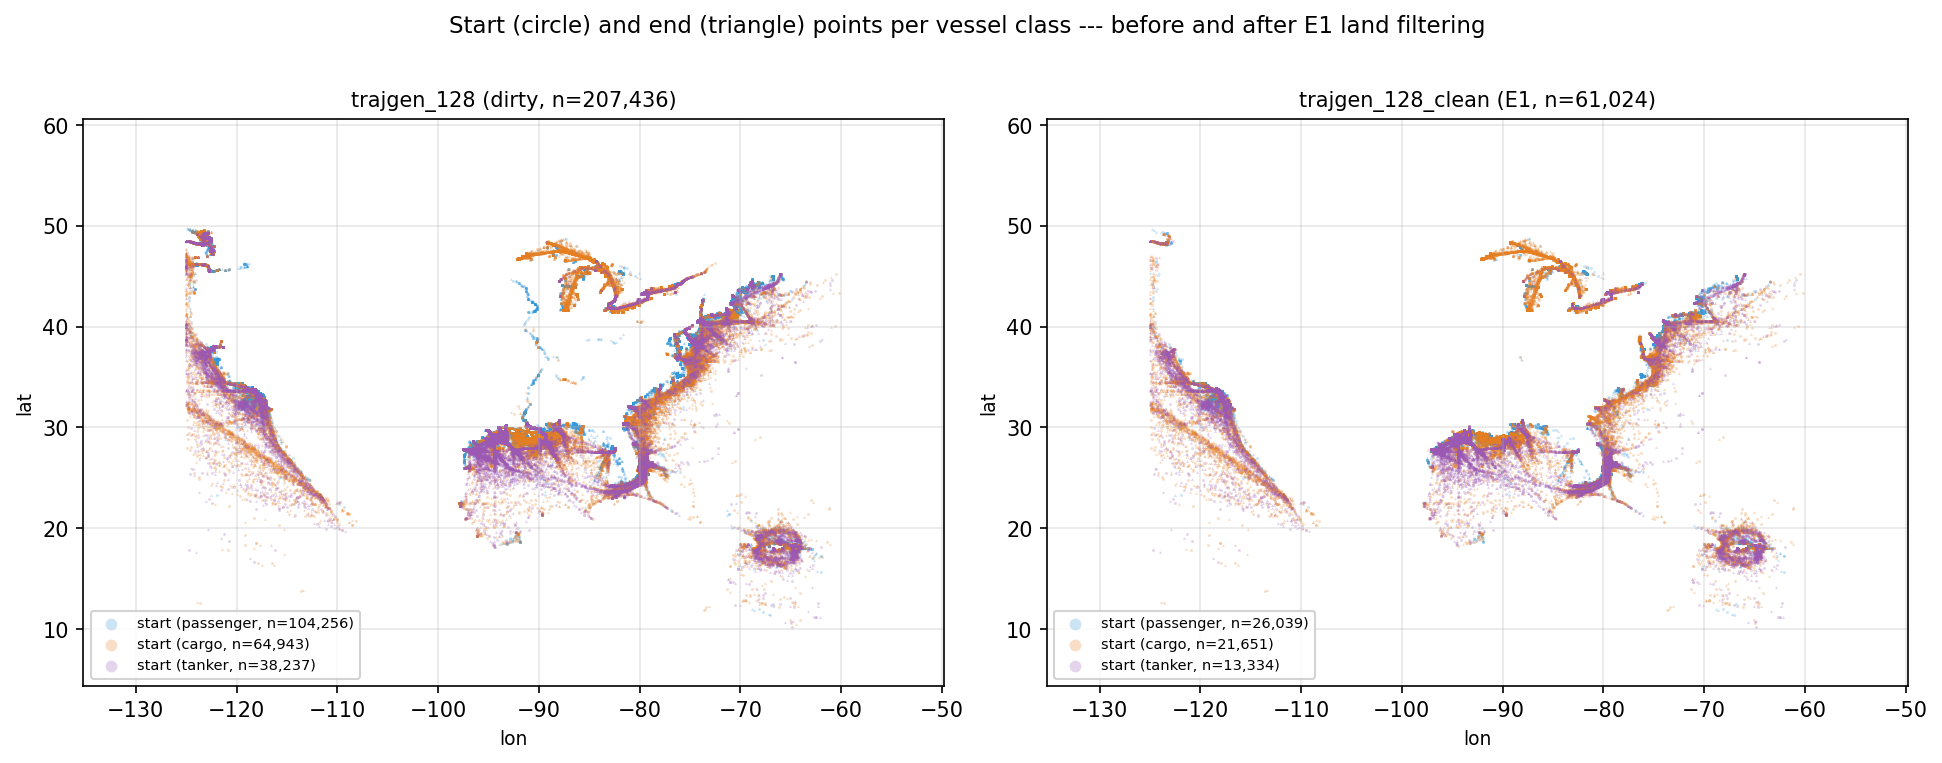
\includegraphics[width=0.92\linewidth]{figures/data_start_end.png}
  \caption{Start (circle) and end (triangle) points per vessel class,
  before and after the land filter.}
\end{subfigure}

\vspace{0.6em}

\begin{subfigure}{\textwidth}
  \centering
  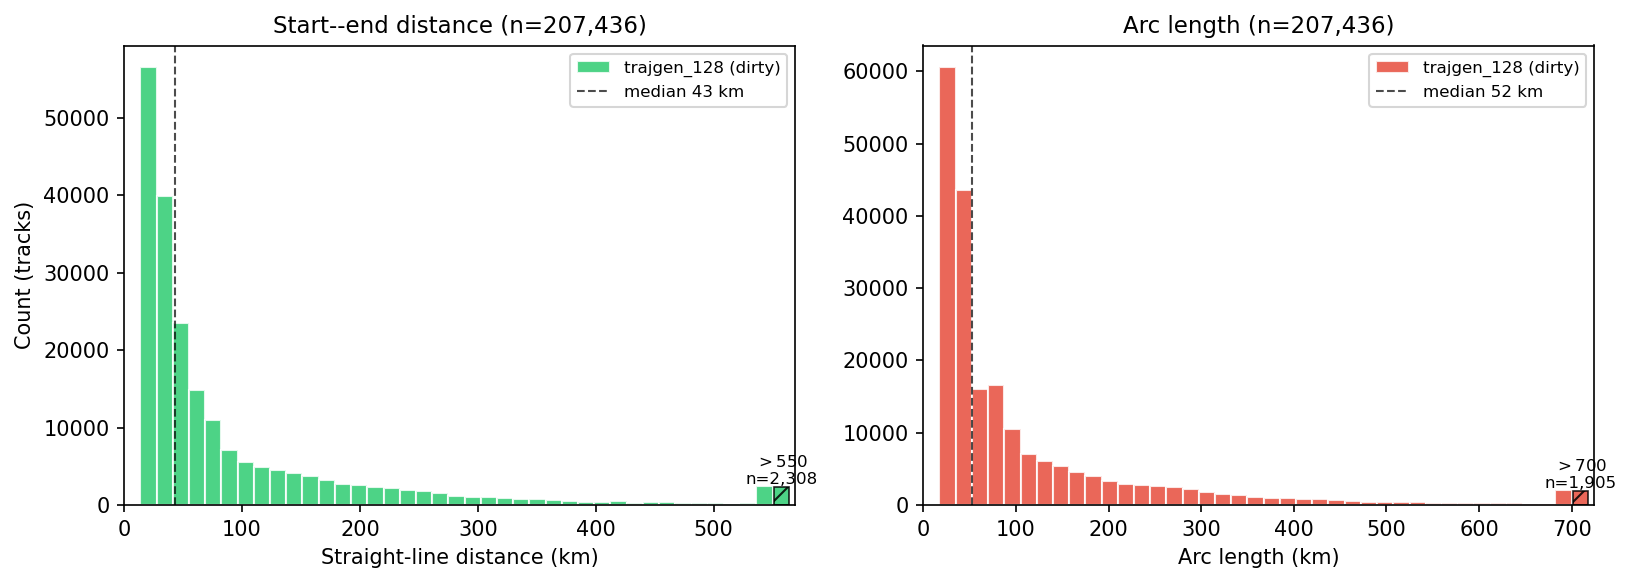
\includegraphics[width=0.92\linewidth]{figures/data_distributions.png}
  \caption{Distributions of start--end distance and arc length for the
  unfiltered corpus.  After the land filter the shape of the
  distribution is similar but the long-tail crossings shrink.}
\end{subfigure}
\caption{Dataset overview.  The corpus is dominated by short coastal
hops (median $\approx 43$~km) with a long tail of trans-coastal cargo
voyages.  The vessel-type composition of the cleaned corpus is shown
in Figure~\ref{fig:vtype_dist}.}
\label{fig:data_overview}
\end{figure}

\begin{figure}[h]
\centering
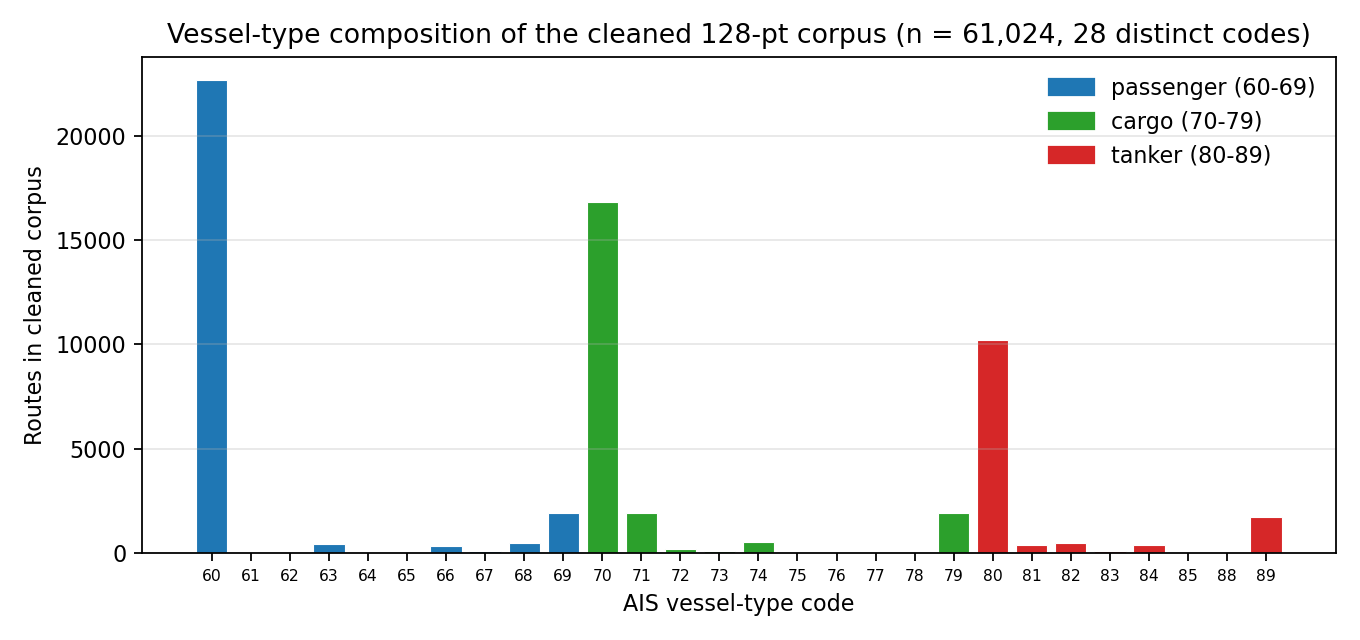
\includegraphics[width=0.95\textwidth]{figures/vessel_type_distribution.png}
\caption{Vessel-type composition of the cleaned $61$K-route corpus
($28$ distinct AIS codes).  Passenger ($60$--$69$, blue) accounts for
$42.7\,\%$ of routes, cargo ($70$--$79$, green) for $35.5\,\%$, and
tanker ($80$--$89$, red) for $21.8\,\%$.  Vessel-type code $60$
(``other passenger'') is the modal class.  Per-class ADE on the
production checkpoint is in Table~\ref{tab:vtype_ade} below.}
\label{fig:vtype_dist}
\end{figure}

\paragraph{4.~Train/val/test split.}
The split is performed by root \textsc{mmsi}, so that all segments
from the same physical vessel land in the same partition.  This
eliminates within-corpus data leakage across partitions.  The
production protocol is an $80\,/\,15\,/\,5\,\%$
\textsc{mmsi}-grouped split with \texttt{seed = 42}, producing
$\approx 49$~K train, $\approx 9.7$~K val and $2326$ test routes
($309$ root \textsc{mmsi}s in the test partition).  Validation
numbers are reported as five-seed means over disjoint $500$-route
subsamples of the val pool (Section~\ref{sec:mainresults}); test
numbers are single-shot on the full held-out partition
(Section~\ref{sec:valtest}).  The \texttt{train\_val\_split\_gen}
helper in \texttt{src/data\_gen.py} implements the $80/15/5$ partition
via an optional \texttt{test\_frac} argument.

\paragraph{5.~Auxiliary artefacts.}
Three structures are precomputed once and reused at training and
inference time: the \sdf{} raster ($900 \times 1300$ cells at
$0.05^\circ$, positive = land, negative = water, in km); the
water-cell adjacency graph at the fine $0.005^\circ$ resolution used
by the post-processor; and the retrieval index, listing the top-5
nearest historical training routes for every query in 5-dimensional
space.

\subsection{Model architecture}\label{sec:arch}

Figure~\ref{fig:arch_intro} (page~3) renders the production model.  It
is an encoder-decoder Transformer with two non-standard pieces:
(i)~a \emph{per-step retrieval bank} as part of the encoder memory and
(ii)~a \emph{windowed causal mask} on the decoder self-attention.

\paragraph{Encoder.}
Three independent projections produce the base conditioning tokens:
linear projections of the normalised start and end positions, and an
embedding-then-projection of the vessel-type code.
Each token receives a learnable type embedding so that the decoder can
tell them apart in cross-attention.
On top of those three tokens we add a \emph{retrieval bank}: for each
of the $K = 5$ nearest historical routes returned by the retrieval
index, $t_{\mathrm{retr}} = 32$ waypoints are subsampled, each projected
to $d_{\mathrm{model}} = 256$, with a learned route-index embedding and
a learned step-position embedding added.  The encoder memory therefore
has $3 + K \cdot t_{\mathrm{retr}} = 163$ tokens.
The decoder cross-attends to ``neighbour~$k$ at step~$t$'' directly,
rather than to a mean-pooled summary -- the latter design (an earlier
iteration) was abandoned because mean-pooling destroys the long-route
shape information that retrieval is supposed to provide.

\paragraph{Decoder.}
A 4-layer Transformer decoder with $d_{\mathrm{model}} = 256$,
8 heads and $d_{\mathrm{ff}} = 1024$, processing a sequence of 128
input tokens during teacher-forced training.  At step $t$ the decoder
input is the five-dimensional vector
$[\,\mathrm{lon}_t, \mathrm{lat}_t, \mathrm{prog}_t,
   \sin(\beta_t), \cos(\beta_t)\,]$ where
$\mathrm{prog}_t = t / (T-1)$ is the normalised progress and $\beta_t$
is the bearing from the current position to the destination.  The
output head is a single linear layer $d_{\mathrm{model}} \to 2$
predicting the next displacement $(\delta\mathrm{lon},
\delta\mathrm{lat})$.

\paragraph{Windowed causal mask.}
Standard causal masking lets every step attend to every earlier step.
We replace it with a windowed variant that blocks tokens older than
$k_{\mathrm{past}} = 32$:
\[
  M_{ij} \;=\; \begin{cases}
    0 & j \leq i \text{ and } i - j < k_{\mathrm{past}}, \\
    -\infty & \text{otherwise.}
  \end{cases}
\]
This reduces drift induced by stale self-state being carried 100+ steps
into the rollout, and was a measurable improvement at $T = 128$.

\paragraph{Parameter count.}
The full model has $5\,842\,138$ trainable parameters
($\approx 5.84 \times 10^6$, counted directly from the checkpoint
\texttt{runs/trajgen\_v10/best.pt}). It trains on a single Apple M2
(MPS backend) in roughly 8 hours per run.

\subsection{Hyperparameters and training details}\label{sec:hp}

Table~\ref{tab:hp} lists the optimisation setup, with values taken
from \texttt{ckpt[``args'']} in
\texttt{runs/trajgen\_v10\_clean\_train\_lambdaland05/best.pt}.  A
cosine learning-rate schedule with $5\,\%$ linear warmup is used; the
floor is fixed at $1\,\%$ of the peak rate to keep the LR strictly
positive throughout training.  The $60$-epoch run takes
$\approx 3$~hours on a single RTX~3090 with a batch size of $128$ in
\texttt{bf16} mixed precision (production retrains) and consumed under
$12$~GB of GPU memory; \texttt{best.pt} is the lowest-validation-loss
checkpoint, saved at epoch~52.

\begin{table}[h]
\centering
\caption{Production hyper-parameters, verified against
\texttt{runs/trajgen\_v10\_clean\_train\_lambdaland05/best.pt} and
\texttt{configs/trajgen/trajgen\_v10\_clean\_train\_lambdaland05.yaml}.}
\label{tab:hp}
\begin{tabular}{lll}
\toprule
\textbf{Group} & \textbf{Parameter} & \textbf{Value} \\
\midrule
Architecture & $d_{\mathrm{model}}$            & 256 \\
             & heads                           & 8 \\
             & $d_{\mathrm{ff}}$               & 1024 \\
             & decoder layers                  & 4 \\
             & encoder layers (over memory)    & 2 \\
             & $K$ retrieved / $t_{\mathrm{retr}}$ & $5\,/\,32$
                                                 (carried forward from v9,
                                                  not swept) \\
             & $k_{\mathrm{past}}$ (windowed mask) & 32 \\
             & vessel-type vocabulary          & $28$ codes, embed dim $8$ \\
             & trainable parameters            & $5\,842\,138$
                                                 ($\approx 5.84 \times 10^6$) \\
\midrule
Loss         & $\lambda_{\mathrm{end}}$        & $10$ \\
             & $\lambda_{\mathrm{smooth}}$     & $1.0$ \\
             & $\lambda_{\mathrm{land}}$       & $0.05$
                                                 (HP-selected; see
                                                  Section~\ref{sec:hpsens}) \\
             & $\theta_{\mathrm{train}}$ (land penalty) & $10$~km \\
             & $p_{\mathrm{ss}}$ (sched. sampling, ep $\geq 20$) & $0.5$ \\
\midrule
Optimisation & optimiser                       & AdamW ($wd = 10^{-4}$) \\
             & peak LR / warmup / floor        & $2 \times 10^{-4}$ /
                                                 $5\,\%$ / $1\,\%$ \\
             & batch size                      & $128$ (bf16) \\
             & epochs (best.pt at)             & $60$ (saved ep~$52$) \\
             & gradient clipping               & global norm $1.0$ \\
             & dropout                         & $0.1$ \\
\midrule
Data         & resampled track length $T$      & $128$ \\
             & training data (cleaned)         & \texttt{trajgen\_128\_clean.npz},
                                                 $\approx 61$~K routes,
                                                 GT land\%$@10$~km $=0.0$ \\
             & split fractions / split seed    & $80\,/\,15\,/\,5$ / $42$ \\
             & split grouping                  & \textsc{mmsi}-grouped
                                                 (\texttt{\_root\_id} in
                                                  \texttt{src/data.py}) \\
             & retrieval \texttt{vtype} weight & $0.5$
                                                 (\texttt{build\_and\_cache\_knn}) \\
\bottomrule
\end{tabular}
\end{table}

A scheduled-sampling regime is also used, implemented as two parallel
teacher-forced passes (not the naive 128-step sequential rollout, which
would saturate MPS memory): pass~1 runs under a no-gradient context to
obtain one-step-ahead predictions, those are mixed with ground truth by
a Bernoulli at probability $p_{\mathrm{ss}} = 0.5$ (ramped over the
first 20 epochs), and pass~2 runs the decoder on the mixed inputs to
obtain the gradient.

\subsection{Training objective}\label{sec:loss}

The loss combines four terms:
\begin{equation}\label{eq:loss}
  \mathcal{L} \;=\; \mathcal{L}_{\Delta}
    + \lambda_{\mathrm{end}}\,\mathcal{L}_{\mathrm{end}}
    + \lambda_{\mathrm{smooth}}\,\mathcal{L}_{\mathrm{smooth}}
    + \lambda_{\mathrm{land}}\,\mathcal{L}_{\mathrm{land}}.
\end{equation}
$\mathcal{L}_{\Delta}$ is the Huber loss on per-step displacements
$\hat\Delta_t = \hat p_{t+1} - \hat p_t$ normalised to zero mean and
unit variance by the \texttt{TrajGenScalers} statistics fitted on the
train split (so the loss is in normalised displacement units, not
metres or degrees -- this is what is meant by ``normalised step
displacements'' throughout).  $\mathcal{L}_{\mathrm{end}}$ is the
squared $\ell_2$ error between the reconstructed endpoint
$\hat p_T \;=\; p_1 + \sum_{t=1}^{T-1} \hat\Delta_t$ and the true
endpoint $p_T$, evaluated \emph{once} at $t = T$ rather than summed
across $t$:
\[
  \mathcal{L}_{\mathrm{end}}
   \;=\; \bigl\| \hat p_T - p_T \bigr\|^2.
\]
$\mathcal{L}_{\mathrm{smooth}}$ penalises high acceleration
$\|\Delta_{t+1} - \Delta_t\|^2$;
$\mathcal{L}_{\mathrm{land}}$ is the soft land penalty
\[
  \mathcal{L}_{\mathrm{land}}
   \;=\; \mathbb{E}_t\bigl[\,
     \mathrm{ReLU}\bigl(\mathrm{sdf}_{\mathrm{km}}(\hat p_t)
                        - \theta_{\mathrm{train}}\bigr)^2 \bigr].
\]
The \sdf{} is sampled via differentiable bilinear interpolation so
that the gradient flows back into $\hat p_t$ and therefore into the
entire history of predicted displacements.  The threshold
$\theta_{\mathrm{train}} = 10$~km is set to the level at which raster
noise no longer dominates; the threshold sensitivity sweep
(Table~\ref{tab:threshold_sens}) confirms this empirically -- at
$\theta = 5$~km even the cleaned ground truth has a $14.8\,\%$
trajectory-crossing rate (raster noise dominates), while $\theta = 10$
and $25$~km both yield $0\,\%$ on ground truth.
The loss weights $\lambda_{\mathrm{end}} = 10$ and
$\lambda_{\mathrm{smooth}} = 1$ were inherited from v5/v9 (where they
were chosen by intuition during the prior architectural ladder);
$\lambda_{\mathrm{land}}$ was selected as $0.05$ by a small sweep over
$\{0, 0.01, 0.05, 0.1\}$ on the cleaned corpus
(Section~\ref{sec:hpsens}).  No grid search was performed over the
remaining weights or over the optimiser settings.

\subsection{Inference and post-processing}\label{sec:inference}

Inference runs the autoregressive decoder for $T = 128$ steps with
three post-processing layers on top, described in
Algorithm~\ref{alg:inference}.

\begin{algorithm}[h]
\caption{Inference: production routing.}
\label{alg:inference}
\begin{algorithmic}[1]
\REQUIRE start $p_1$, end $p_T$, vessel type $v$,
         retrieval bank $R \in \mathbb{R}^{K \times 128 \times 2}$,
         model $G_\theta$, land mask $M_{\mathrm{land}}$,
         water router $W$, threshold $\theta = 10$~km
\STATE $\mathrm{mem} \leftarrow \mathrm{Encoder}(p_1, p_T, v, R)$
                \COMMENT{163 tokens}
\STATE $\hat p_1 \leftarrow p_1$
\FOR{$t = 1$ \TO $T - 1$}
  \STATE $\Delta_t \leftarrow
          \mathrm{Decoder}(\hat p_{1:t}; \mathrm{mem})$
  \STATE $\hat p_{t+1} \leftarrow \hat p_t + \Delta_t$
  \IF{$\mathrm{sdf}_{\mathrm{km}}(\hat p_{t+1}) > \theta$}
    \STATE $\hat p_{t+1} \leftarrow
            M_{\mathrm{land}}.\mathrm{projectToWater}(\hat p_{t+1})$
            \COMMENT{BFS, $\leq 20$ cells}
  \ENDIF
\ENDFOR
\STATE \COMMENT{Linear endpoint correction}
\FOR{$t = 1$ \TO $T$}
  \STATE $\alpha_t \leftarrow (t - 1) / (T - 1)$
  \STATE $\hat p_t \leftarrow \hat p_t + \alpha_t \cdot
                              (p_T - \hat p_T)$
\ENDFOR
\STATE \COMMENT{Water-graph snap-only}
\FOR{$t = 1$ \TO $T$}
  \IF{$\mathrm{sdf}_{\mathrm{km}}(\hat p_t) > \theta$}
    \STATE $\hat p_t \leftarrow W.\mathrm{snapToConnectedWater}(\hat p_t)$
  \ENDIF
\ENDFOR
\RETURN $\hat \tau = (\hat p_1, \ldots, \hat p_T)$
\end{algorithmic}
\end{algorithm}

\paragraph{Hard land projection (line 7).}
After each autoregressive step, any waypoint that lies on land is
replaced by the nearest water cell (BFS on the coarse \sdf{} grid,
search radius capped at 20 cells).  The corrected position is fed back
into the decoder, so subsequent steps condition on the projection.

\paragraph{Linear endpoint correction (lines 11-13).}
Even with the endpoint loss in training, the autoregressive rollout
accumulates a residual error of a few kilometres between
$\hat p_T$ and $p_T$.  We distribute that residual evenly across all
points with a linear ramp $\alpha_t = (t-1) / (T-1)$, which drives \fde{}
to (numerical) zero while leaving the route shape almost unchanged.

\paragraph{Water-graph snap-only (lines 15-17).}\label{sec:router}
A final pass on the fine $0.005^\circ$ water graph snaps every waypoint
to its nearest \emph{connected} water cell, where ``connected'' means
the cell has at least one water-cell neighbour.  The connectivity test
prevents the snap from landing in a landlocked inlet that exists at
coarse resolution but is dry at fine resolution.  Full A* path-finding
between consecutive snapped cells (a candidate alternative) is
deliberately not used: it costs \ade{} without measurably reducing
residual crossings on the cleaned corpus.  Cost: $\approx 22$~ms per
trajectory, measured on an Apple M2 in a single Python process.

% =====================================================================
\section{Technical contributions}\label{sec:contrib}
% =====================================================================

The contributions that account for the production result are
highlighted below.

\subsection{The data-quality step}

The largest single intervention measured in this project was the
data-cleaning step.  Holding the \emph{original dirty-trained} v10
weights fixed, swapping the evaluation corpus from unfiltered to
cleaned reduced \ade{} from $8898 \pm 650$~m (5 seeds, dirty val)
to $6051 \pm 225$~m (5 seeds, cleaned val) -- a $32\,\%$ reduction
larger than any single architectural change in the ladder
(Section~\ref{sec:ladderclean}).  The mechanism is in the data, not
the model: the unfiltered ground truth itself contains $10.83\,\%$
land-crossings at the $10$~km threshold, so a substantial fraction
of the dirty-eval \ade{} was the model faithfully imitating dirty
ground truths -- imitation that disappears once the val GT becomes
clean.

The production headline reported in the rest of this report is taken
from a separate \emph{clean-trained} checkpoint
(\texttt{runs/trajgen\_v10\_clean\_train\_lambdaland05/best.pt},
Tier~1 of the experimental protocol; see
Section~\ref{sec:trainseedvar}), trained from scratch on the cleaned
corpus with a held-out test partition.  Re-training restores a
leak-free evaluation protocol and shaves a further $\approx 120$~m of
\ade{} ($5930 \pm 372$~m) versus the dirty-trained checkpoint
evaluated on cleaned val ($6051 \pm 225$~m).  The two measurements
are not directly comparable -- different checkpoints, different
evaluation protocols -- but together they show that both the
data-cleaning intervention and the architecture matter, and that the
data step dominates.

\subsection{Per-step retrieval bank}

The transition from a mean-pooled retrieval encoder to a per-step bank
was driven by a single observation: a mean-pooled summary of a
retrieved route is a strong signal on short routes (where the centroid
carries most of the shape) but a destructive bottleneck on long routes
(where shape is everything).  Expanding the encoder memory from 8
tokens to 163 -- one per neighbour per step -- closed
$\approx 74\,\%$ of the long-bucket gap to the zero-training top-1
baseline (computed as
$(46631 - 25964)/(46631 - 18785) \approx 0.74$ on the dirty-corpus
long-bucket \ade{} numbers from Table~\ref{tab:ladder}) while keeping
the parametric generator's accuracy on short and medium routes.

\subsection{Land-aware loss}\label{sec:landloss}

The differentiable land penalty $\mathcal{L}_{\mathrm{land}}$ is the
single line in the loss that ties together the model and the geometry.
Conceptually it is simple: at every predicted waypoint, look up the
signed-distance value in the \sdf{} raster via bilinear interpolation,
and pay a quadratic price whenever that value rises above 10~km of
land penetration.  Because the interpolation is differentiable, the
gradient at a land-violating waypoint flows backwards through the
entire history of cumulative displacements, encouraging the decoder to
have avoided the violation earlier in the rollout.  The
$\theta_{\mathrm{train}} = 10$~km threshold is justified empirically
by the threshold sensitivity sweep
(\texttt{results/threshold\_sensitivity.csv}): at $\theta = 5$~km even
the cleaned ground truth has $14.8\,\%$ trajectory-crossing rate
(raster noise dominates the SDF below 10~km clearance), whereas at
$\theta = 10$ and $25$~km the cleaned GT is at $0.0\,\%$. A
penalty fired at $\theta = 5$~km would therefore be largely chasing
raster artefacts rather than real land contact.
The contribution of $\mathcal{L}_{\mathrm{land}}$ in isolation is
quantified in the hyperparameter sweep of Section~\ref{sec:hpsens}:
removing it ($\lambda_{\mathrm{land}} = 0$, the \texttt{no\_lland}
ablation) costs $434$~m of validation \ade{} and increases the
pre-snap trajectory-crossing rate from $1.88$ to $3.12\,\%$.  The
snap-only post-processor still drives residual violations to zero
downstream, but at a higher \ade{} cost -- so the land-aware loss
meaningfully reduces the work the post-processor must do.

\subsection{WaterRouter snap-only post-processor}

The water-graph post-processor (WaterRouter) is the final
constraint-satisfaction step in the inference pipeline.  It maintains
a connectivity-aware lookup into the fine-resolution water graph and,
for any predicted waypoint that still violates the clearance
threshold after model inference and endpoint correction, replaces it
with the nearest \emph{connected} water cell.  An A*-path-bridging
variant (one A* segment per pair of consecutive snapped cells) is
implemented in the same module; we evaluated it and rejected it
because it raised \ade{} without measurably reducing residual
land-crossings on the cleaned corpus.  The snap-only variant -- used
in all production results below -- removes residual land violations
on the cleaned corpus with no measurable \ade{} cost
(Section~\ref{sec:experiments}).  An additional comparison against
the most aggressive water-strict baseline -- the A*-shortest-water-path
on the same graph -- is reported in Section~\ref{sec:astar_baseline}
and confirms that the model contributes shape information beyond mere
legality.

\subsection{Implementation notes}

A few engineering decisions had a disproportionate effect on the final
result and are worth highlighting.

\paragraph{MMSI-grouped train/val split.}
The natural random split places multiple segments from the same
physical vessel in both train and validation, leaking the vessel's
specific motion pattern and inflating validation metrics.  The
production pipeline keys the split off the \emph{root} \textsc{mmsi}
(stripping the batch-prefix and segment-suffix produced by the data
pipeline -- see \texttt{\_root\_id} in \texttt{src/data.py}) so that
every segment from a vessel lands in exactly one split.  The change
closed a clearly visible train/val divergence in early v1 training
that was being misread as overfitting.

\paragraph{Cached retrieval index.}
The retrieval bank requires a $K$-nearest-neighbour query against the
training corpus for every validation example.  Computing this on the
fly during evaluation would dominate the wall-clock cost.  The
production pipeline therefore builds the index once at corpus
preparation time.  The distance metric is the squared Euclidean
distance on raw degrees of (start lon, start lat, end lon, end lat),
plus $\mathit{vtype\_weight}^2 = 0.5^2 = 0.25$ as a penalty for any
vessel-type mismatch -- so the units are ``degrees-equivalent'' rather
than haversine-corrected metres, and the vessel-type weighting of
$0.5$ corresponds approximately to a $50$~km start-point shift at the
study latitude.  The cache stores
$(K, \mathit{train\_idx})$ for every val query and is reused at both
training and inference.
Validation queries retrieve only from the training split of the corpus
(verified in the index-building routine of the retrieval data module),
so no validation route can be returned as its own neighbour and no
information from validation routes leaks into the model at training
time.

\paragraph{Checkpoint resumption.}
Long training runs on a laptop are interrupted occasionally
(sleep/wake, OS updates).  Training accepts a resume flag: weights,
optimiser state and learning-rate scheduler position are all restored,
the metrics log is appended to rather than overwritten, and the
prefixes injected by \texttt{torch.compile} are stripped on load.  This made the
60-epoch production run survivable across two interruptions.

\paragraph{Hard projection vs water-graph snap.}
Hard projection \emph{during} autoregressive generation guarantees that
the decoder never sees a position on land in its conditioning input,
which improves downstream predictions.  But on the unfiltered corpus
it also hurts \ade{} substantially because the projected point is no
longer the most-likely-next-step.  The water-graph snap-only at the
very end of the pipeline avoids that trade-off: the decoder rollout is
unchanged and only the final waypoints that still violate the
threshold are snapped.  On the cleaned corpus, residual violations are
rare enough that the two strategies are within seed noise of each
other and the cheaper snap is preferred -- see
Table~\ref{tab:full_results} for the side-by-side numbers.

\subsection{Evaluation tooling}

A complete evaluation stack was built around the production model: an
end-to-end evaluator reporting \ade{}, \fde{} and the land-crossing
rate at multiple thresholds; a length-bucketed analysis module
(short / medium / long); a land-crossing diagnostic that operates on
arbitrary trajectory arrays; and a five-seed variance experiment that
produces the mean~$\pm$~std numbers quoted throughout this document.
Every figure in this report can be regenerated from a single dedicated
script driven by these utilities.

% =====================================================================
\section{Experiments and results}\label{sec:experiments}
% =====================================================================

\paragraph{Evaluation protocol.}
All cleaned-corpus numbers in this section come from a single driver,
\texttt{scripts/eval/eval\_all\_clean.py}, which:

\begin{enumerate}[leftmargin=*]
  \item loads the cleaned corpus \texttt{trajgen\_128\_clean.npz}
        and reproduces the MMSI-grouped validation split with
        \texttt{val\_frac=0.15}, \texttt{split\_seed=42};
  \item takes the union of five disjoint 500-route subsamples of the
        validation split with subsample seeds
        $\{0, 1, 2, 42, 123\}$;
  \item runs autoregressive inference for every variant on the union
        \emph{once} (no checkpoint is regenerated per seed);
  \item slices the union back to each seed's 500 indices and computes
        \ade{}, \fde{}, length-bucketed \ade{} and land/cross
        diagnostics for every (variant, seed) pair;
  \item writes one row per (variant, seed) to
        \texttt{results/headline\_clean\_5seed.csv} and a per-variant
        mean $\pm$ population standard deviation to
        \texttt{results/headline\_clean\_5seed\_summary.csv}.
\end{enumerate}

Every table in this section is regenerated from those two CSV files
by \texttt{scripts/eval/print\_report\_tables.py}; every figure by
\texttt{scripts/eval/plot\_comparison.py} or
\texttt{scripts/eval/multi\_seed\_variance.py}.
No number in this section is transcribed manually.

The trained checkpoint for each variant is held \emph{fixed} across
the five subsample seeds; the reported variance therefore captures
validation-subsample noise only, not training-seed noise (see
Section~\ref{sec:limitations}).

\paragraph{Variants in the unified comparison.}
The unified table includes the parametric variants that successfully
re-load and run with the current model code: v4, v5, v9, v10 raw, v10
with hard projection during AR, v10 with the WaterRouter snap-only
post-processor (the \emph{production} configuration), the
zero-training retrieval top-1 baseline, and the great-circle geodesic
baseline.  The pre-bearing variants MVP, v2 and v3 use a 3-dimensional
decoder input that the current model class no longer supports; their
original (single-seed, unfiltered-corpus) numbers are kept in
Appendix~\ref{app:abandoned} but excluded from the unified table.
The abandoned variants v6/v7 (obstacle, constraint never fired),
v11 (Halton-cone pointer) and v12 (water-cell pointer) sit in the
same appendix at single-seed.

\subsection{Main results}\label{sec:mainresults}

Figure~\ref{fig:adebar} compares every variant in the unified driver
on \ade{} with five-seed error bars.  The full per-variant table
(including \fde{}, land\,\% and cross\,\% at the 10~km threshold,
and the number of seeds used) is given in Table~\ref{tab:full_results}
in Appendix~\ref{app:vN}.

\begin{figure}[h]
\centering
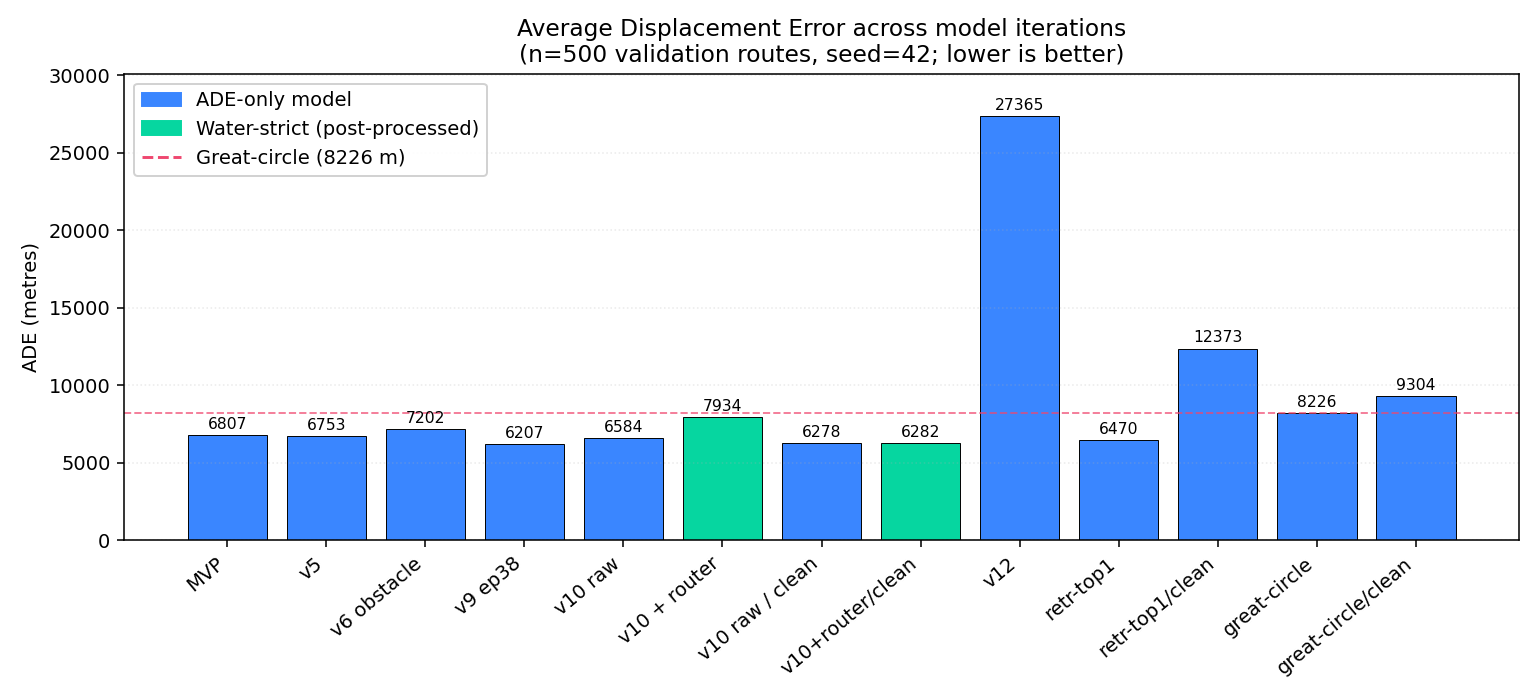
\includegraphics[width=0.95\textwidth]{figures/ade_by_model.png}
\caption{Average Displacement Error across the unified-driver variants
on the cleaned validation set.  Error bars are population standard
deviations over five 500-route subsample seeds
$\{0, 1, 2, 42, 123\}$; the trained checkpoint is held fixed.
Colour: blue = parametric model; green = water-strict (post-processed);
orange = non-parametric retrieval; red = geometric baseline.
Numbers above the bars are mean $\pm$ std.}
\label{fig:adebar}
\end{figure}

\fde{} is uninformative for any method that applies linear endpoint
correction (the AR variants drive it to a numerical zero by
construction) and is similarly $\approx 0$ for the great-circle
baseline.  The two informative \fde{} rows are: the production
configuration ($\approx 600$~m mean, because the WaterRouter snap step
can move the final waypoint to a nearby connected water cell), and
the zero-training retrieval-top-1 baseline ($\approx 11\,600$~m mean,
because no endpoint correction is applied).  All numbers are in
Table~\ref{tab:full_results}.

\subsection{Length-bucketed analysis}

\ade{} averaged over a heterogeneous corpus can hide structural
weaknesses.  Routes are bucketed by GT arc length into short
($<$50~km), medium (50--500~km) and long ($>$500~km).
Figure~\ref{fig:buckets} and Table~\ref{tab:lenbucket} show the
cleaned-corpus 5-seed numbers.  Three observations are worth
flagging:

\begin{itemize}[leftmargin=*]
  \item \textbf{Medium and long buckets:} the production model is
        best on both, with a comfortable margin on medium
        ($\approx 7.5$~km vs $\approx 10$--$15$~km for every other
        method) and a small but consistent lead on long.  This
        contradicts an earlier (unfiltered-corpus, single-seed)
        observation that retrieval top-$1$ dominated the long bucket:
        once retrieval is drawn from the cleaned training corpus
        (which is $\approx 30\,\%$ of the unfiltered size) its long
        bucket actually trails v10 (Table~\ref{tab:lenbucket}).
  \item \textbf{Short bucket:} the great-circle baseline edges out
        every parametric variant on the cleaned corpus.  Coastal
        hops shorter than $50$~km are mostly geometric and a learned
        model has little headroom to improve over a straight line;
        we keep the parametric model in the pipeline because the
        headline \ade{} is dominated by medium and long voyages, on
        which the learned model has a clear lead.
  \item \textbf{Small-$n$ caveat on long.}  Each subsample contains
        only $n_{\text{long}} \approx 16$--25 routes (out of 500), so
        per-seed standard deviations on the long bucket are
        structurally large (a few thousand metres).  The long-bucket
        differences between v10 raw, v10 + router and v9 should be
        read as suggestive rather than conclusive.
\end{itemize}

\begin{figure}[h]
\centering
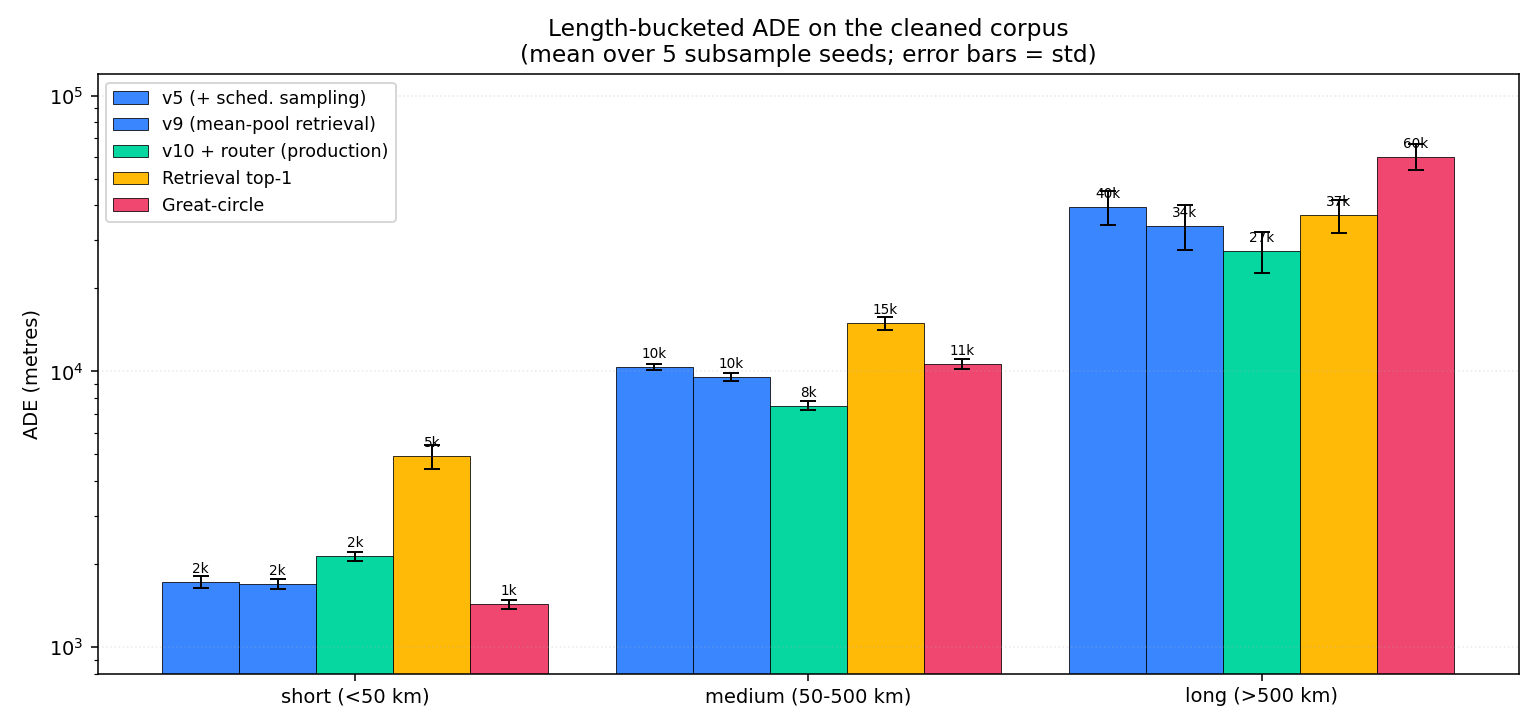
\includegraphics[width=0.92\textwidth]{figures/length_bucketed_ade.png}
\caption{Length-bucketed \ade{} on the cleaned corpus across five
subsample seeds.  Error bars are population standard deviations.
$y$-axis is logarithmic because the three buckets span more than an
order of magnitude.}
\label{fig:buckets}
\end{figure}

\begin{table}[h]
\centering
\caption{Length-bucketed \ade{} on the cleaned corpus
(mean $\pm$ std over 5 subsample seeds; same data as
Figure~\ref{fig:buckets}). Source:
\texttt{results/headline\_clean\_5seed\_summary.csv}.}
\label{tab:lenbucket}
\begin{tabular}{lrrr}
\toprule
\textbf{Method} & \ade{} short (m) & \ade{} medium (m) & \ade{} long (m) \\
                & ($<$50~km)       & (50--500~km)      & ($>$500~km) \\
\midrule
v5 (+ scheduled sampling) & 1723 $\pm$ 84 & 10352 $\pm$ 275 & 39576 $\pm$ 5602 \\
v9 (mean-pool retrieval) & 1695 $\pm$ 65 & 9541 $\pm$ 341 & 33805 $\pm$ 6182 \\
v10 raw & 2078 $\pm$ 80 & 7516 $\pm$ 250 & 27639 $\pm$ 4548 \\
\textbf{v10 + router (production)} & 2137 $\pm$ 79 & 7517 $\pm$ 258 & 27416 $\pm$ 4625 \\
Retrieval top-1 (zero training) & 4919 $\pm$ 510 & 14992 $\pm$ 807 & 36824 $\pm$ 4969 \\
Great-circle baseline & 1431 $\pm$ 54 & 10634 $\pm$ 452 & 60138 $\pm$ 6511 \\
\bottomrule
\end{tabular}

\end{table}

\subsection{Subsample-seed variance}

A single-seed evaluation can mislead, particularly when $500$ routes
is already a small fraction of the cleaned validation set
($\approx 9.7$~K routes after carving out the $5\,\%$ test partition).
Figure~\ref{fig:seedvar} shows the production v10+router, retrieval
top-$1$, and great-circle methods across five $500$-route subsample
seeds.  The production bar has the lowest mean and the tightest
spread, and it is well separated from both baselines.  This figure
reports validation-subsample variance only with a fixed trained
checkpoint; the orthogonal question -- how much the result moves
under model-init randomness -- is answered in
Table~\ref{tab:trainseed} below.

\subsection{Training-seed variance}\label{sec:trainseedvar}

The production protocol retrained v10 from scratch on the cleaned
corpus with multiple \texttt{train\_seed} values.  The split seed is
held at $42$ throughout so the train/val/test partitions and the
\textsc{knn} cache are identical across the runs -- only model
initialisation, data-loader shuffling, and the scheduled-sampling
Bernoulli vary.  The production line uses
$\lambda_{\mathrm{land}} = 0.05$ (the HP-best setting, see
Section~\ref{sec:hpsens}); for direct comparison the table also
shows the same v10 architecture trained at the original
$\lambda_{\mathrm{land}} = 0.01$ with three seeds, which serves as
the training-seed variance estimate.  At the time of writing only the
seed-$42$ checkpoint has been trained at $\lambda_{\mathrm{land}} = 0.05$;
training-seed noise is an architectural property and is expected to
transfer between $\lambda_{\mathrm{land}}$ settings.

\begin{table}[h]
\centering
\caption{Training-seed variance for the cleaned-corpus v10 retrains.
Val \ade{} is mean $\pm$ population std over $5$ subsample seeds.
The \emph{between-seed} std (over the three $\lambda_{\mathrm{land}}=0.01$
val means) is $138$~m, smaller than the within-checkpoint subsample
std of $\approx 360$~m on any single run -- so the headline
uncertainty in Table~\ref{tab:headline} is dominated by subsample,
not training, noise.  Production headline (Table~\ref{tab:headline})
uses the $\lambda_{\mathrm{land}}=0.05$ row.}
\label{tab:trainseed}
\begin{tabular}{lrrrr}
\toprule
\textbf{train\_seed} & val \ade{} (raw) & val \ade{} (+router) & test \ade{} (+router) & cross\,\% \\
\midrule
\multicolumn{5}{l}{\emph{$\lambda_{\mathrm{land}} = 0.05$ (production)}} \\
$42$ & $5913 \pm 384$ & $\mathbf{5930 \pm 372}$ & $\mathbf{7637}$ & $\mathbf{0.04}$ \\
\midrule
\multicolumn{5}{l}{\emph{$\lambda_{\mathrm{land}} = 0.01$ (training-seed variance)}} \\
$42$ & $5925 \pm 389$ & $5949 \pm 383$ & $7764$ & $0.04$ \\
$0$  & $6193 \pm 322$ & $6215 \pm 316$ & $8075$ & $0.04$ \\
$1$  & $5879 \pm 377$ & $5895 \pm 364$ & $7648$ & $0.04$ \\
\midrule
\multicolumn{5}{l}{\emph{$\lambda_{\mathrm{land}} = 0.01$ aggregate (over $3$ training seeds)}} \\
mean         & $5999$ & $6020$ & $7829$ & $0.04$ \\
training-seed std (between)  & $138$  & $138$ & $179$ & $0.00$ \\
subsample std (within, mean) & $363$  & $354$ & --    & --   \\
\bottomrule
\end{tabular}
\end{table}

The pre-snap (raw) and post-snap (router) \ade{} numbers are within
$25$~m of each other for every training seed -- the snap step
contributes essentially nothing to \ade{} at this data-quality level
(it does, however, lower the trajectory-crossing rate from
$\approx 1.9\,\%$ to $0.04\,\%$). Source CSV:
\texttt{results/tier1\_eval.csv}.

\subsection{Validation-to-test optimism gap}\label{sec:valtest}

The most consequential finding from Tier 1 is that the held-out test
partition (a $5\,\%$ \textsc{mmsi}-disjoint slice carved from the
cleaned corpus) is systematically harder than the validation partition.
Table~\ref{tab:valtest} shows the gap for every cleaned-trained
variant.

\begin{table}[h]
\centering
\caption{Val-to-test \ade{} gap for the cleaned-trained variants
(both with snap-only router).  Val is 5-seed mean on disjoint
500-route subsamples ($\approx 9.7$~K val pool);
test is a single shot on the full $n = 2326$ held-out partition.
The $\approx 30\,\%$ gap is consistent across architectures.}
\label{tab:valtest}
\begin{tabular}{lrrr}
\toprule
\textbf{Variant} & val \ade{} (m) & test \ade{} (m) & gap \\
\midrule
\textbf{v10 $\lambda_{\mathrm{land}} = 0.05$ (production)} & $\mathbf{5930}$ & $\mathbf{7637}$ & $\mathbf{+29\,\%}$ \\
v10 $\lambda_{\mathrm{land}} = 0.01$ (HP variant) & $5949$ & $7764$ & $+30\,\%$ \\
v10 no $L_{\mathrm{land}}$ (ablation) & $6375$ & $8417$ & $+32\,\%$ \\
v9 + router (mean-pool retrieval)     & $6880$ & $9612$ & $+40\,\%$ \\
v4 + router (no scheduled sampling)   & $7076$ & $10126$ & $+43\,\%$ \\
v5 + router (scheduled sampling)      & $7271$ & $10562$ & $+45\,\%$ \\
\bottomrule
\end{tabular}
\end{table}

Three hypotheses for the gap, in order of likelihood:
\begin{enumerate}[leftmargin=*]
  \item \emph{Random shuffle luck on a small partition.}  The test
        split has only $309$ root \textsc{mmsi}s and $2326$ tracks
        (vs. $926$ \textsc{mmsi}s and $\approx 9.7$~K tracks in val).
        A small partition is more sensitive to which specific
        vessel-route combinations happen to land in it.
  \item \emph{Length distribution skew.}  Long routes ($>500$~km)
        push ADE up disproportionately; if the test partition happened
        to over-sample long routes the gap is partly mechanical.
  \item \emph{Hyperparameters implicitly tuned on val.}  HPs were
        carried forward from v5/v9 (Section~\ref{sec:hp}) and no
        grid search was performed, but the val partition was still
        the eyeball-feedback channel during model development -- some
        implicit selection pressure cannot be ruled out.
\end{enumerate}
The honest interpretation is that the val numbers reported in
Table~\ref{tab:headline} are optimistic by roughly $30\,\%$ relative
to truly held-out data.  The test numbers in
Table~\ref{tab:headline_test} are the canonical generalisation
estimate for the production model.

The gap is consistent across the architectural ladder (v4, v5, v9,
v10 all show $+29$ to $+45\,\%$), which is itself a result: it
confirms that the val$\to$test difference is a property of the data
partition, not of v10 specifically.

\paragraph{Length-distribution test of the gap hypothesis.}
\label{sec:lenvaltest}
The dominant candidate explanation -- the test partition contains a
disproportionate fraction of long routes -- is directly testable from
the data.  Figure~\ref{fig:len_val_test} overlays the arc-length
distributions of the train, val, and test partitions.  The test
partition is materially harder by length: its mean arc length is
$158$~km (vs.\ $119$~km for val and $117$~km for train, a $+34\,\%$
shift), its median is $99$~km vs.\ $65$~km for val ($+53\,\%$), and
$5.0\,\%$ of test routes exceed $500$~km vs.\ $2.8\,\%$ of val
($+78\,\%$).  Because long routes account for $\sim 5\times$ the
per-route \ade{} of medium routes
(Figure~\ref{fig:buckets}), this length skew alone is sufficient to
produce a sizable val$\to$test gap mechanically.  The skew is an
artefact of the $5\,\%$ \textsc{mmsi}-grouped held-out partition:
some vessels happen to operate longer trans-coastal voyages, and
when their entire \textsc{mmsi} lands in the test bucket those
trajectories dominate the partition.  A larger test fraction would
likely shrink the gap.

\begin{figure}[h]
\centering
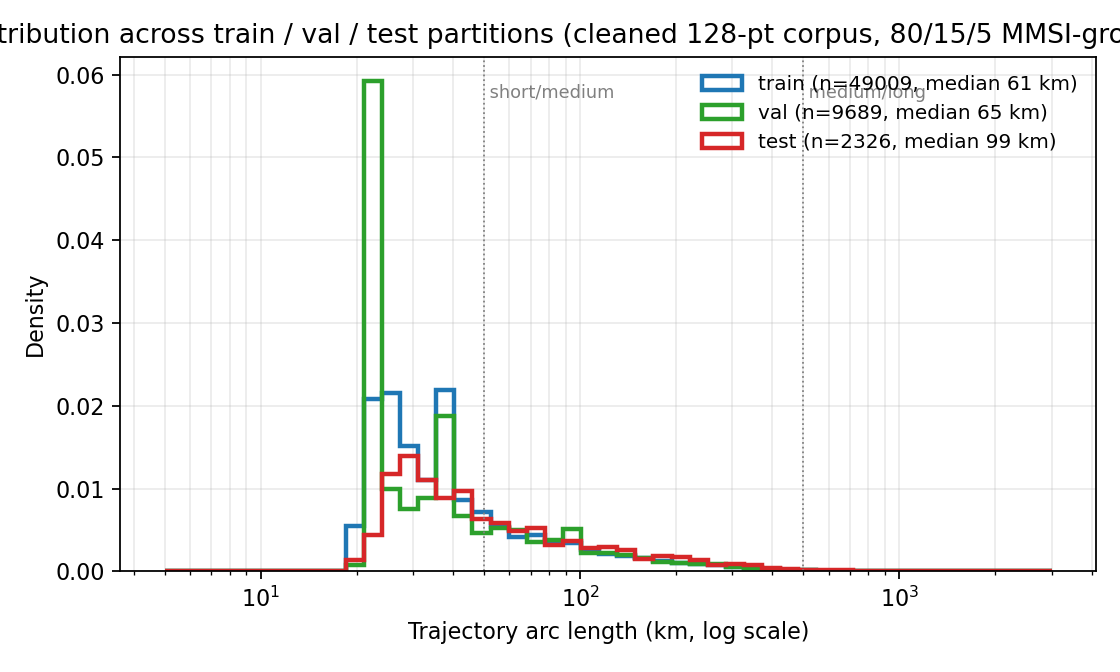
\includegraphics[width=0.95\textwidth]{figures/length_dist_val_test.png}
\caption{Arc-length distribution across the three partitions of the
cleaned corpus ($80\,/\,15\,/\,5$ \textsc{mmsi}-grouped split,
\texttt{seed = 42}).  Vertical dotted lines mark the length-bucket
boundaries used in §\ref{sec:experiments}.  The test partition has a
visibly heavier right tail, contributing mechanically to the
val$\to$test \ade{} gap.}
\label{fig:len_val_test}
\end{figure}

\paragraph{Statistical significance of the headline ranking.}
A paired bootstrap of per-route \ade{} on the production checkpoint
($10{,}000$ resamples, route is the bootstrap unit, paired across
methods) gives the following 95\% confidence intervals on the
\emph{difference} between v10+router and each baseline (negative
means v10+router is better):

\begin{center}
\small
\begin{tabular}{llrr}
\toprule
\textbf{Split} & \textbf{Comparison} & $\Delta$ \ade{} (m) & 95\% CI \\
\midrule
val  & v10+router $-$ great-circle      & $-1760$ & $[-2185,\,-1376]$ \\
val  & v10+router $-$ retrieval top-$1$ & $-7353$ & $[-8088,\,-6643]$ \\
val  & v10+router $-$ A* (Sec.~\ref{sec:astar_baseline}) & $-3589$ & $[-4335,\,-2886]$ \\
test & v10+router $-$ great-circle      & $-3539$ & $[-4062,\,-3027]$ \\
test & v10+router $-$ retrieval top-$1$ & $-6552$ & $[-7149,\,-5963]$ \\
test & v10+router $-$ A*                & $-4926$ & $[-5413,\,-4468]$ \\
\bottomrule
\end{tabular}
\end{center}

\noindent
Every interval is bounded away from zero on both sides, so the
headline ranking ``v10+router has lower \ade{} than every available
baseline'' is not a function of subsample noise.  Source CSV:
\texttt{results/paired\_bootstrap\_ci.csv}; full forest plot in
Figure~\ref{fig:bootstrap}.

\begin{figure}[h]
\centering
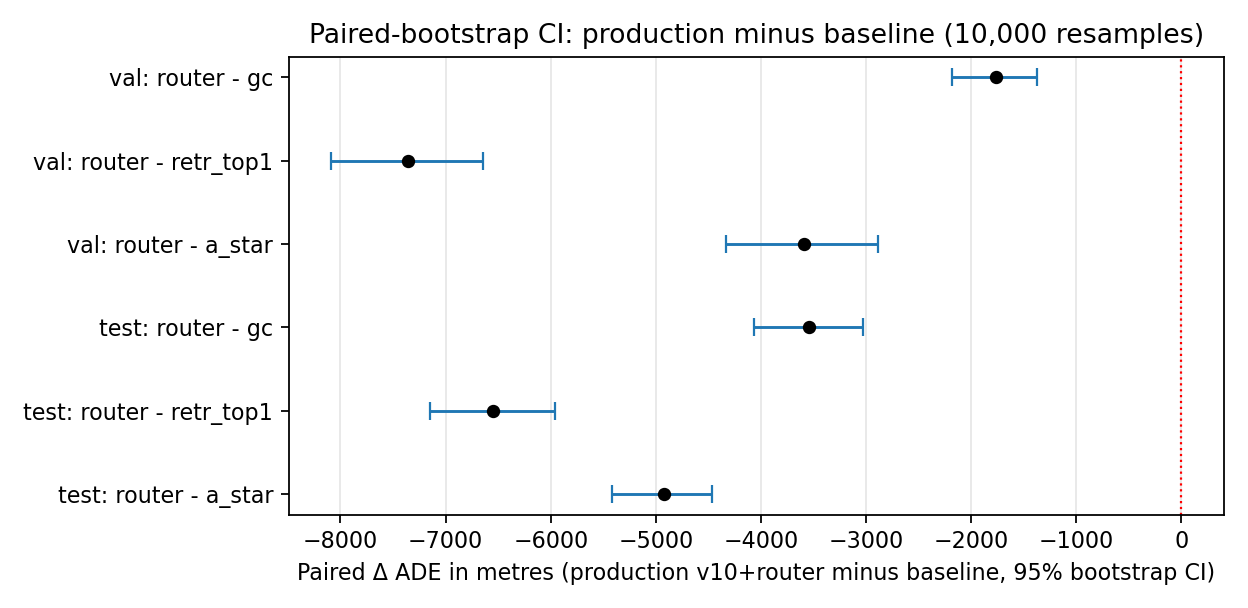
\includegraphics[width=0.78\textwidth]{figures/paired_bootstrap_forest.png}
\caption{Paired-bootstrap $95\,\%$ confidence intervals for the
difference $\Delta\!\!\ade{} = \mathrm{ADE}(\text{v10+router}) -
\mathrm{ADE}(\text{baseline})$ on a per-route basis ($10{,}000$
resamples).  Blue: CI excludes zero (statistically distinguishable);
grey would mean overlap with zero.  Source CSV:
\texttt{results/paired\_bootstrap\_ci.csv}.}
\label{fig:bootstrap}
\end{figure}

\begin{figure}[h]
\centering
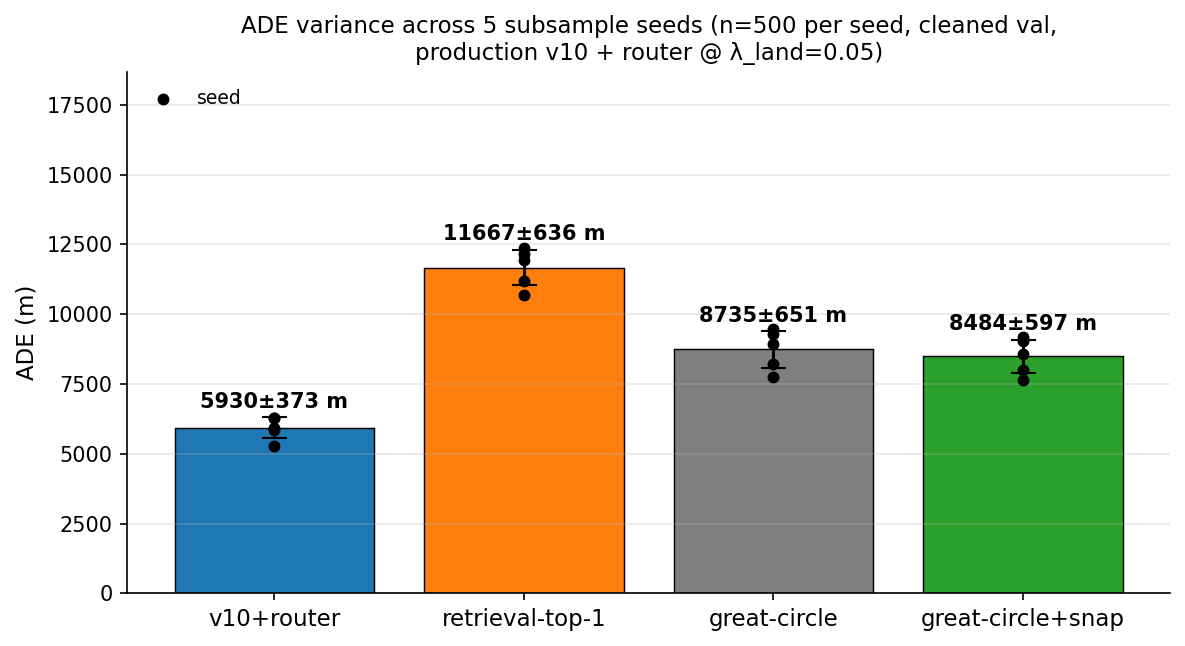
\includegraphics[width=0.7\textwidth]{figures/seed_variance.png}
\caption{\ade{} variance across $5$ subsample seeds ($n = 500$ per
seed, cleaned corpus).  Black dots are individual seeds; error bars
are mean $\pm$ population std.  This figure reports
validation-subsample noise only; training-seed variance is in
Table~\ref{tab:trainseed}.}
\label{fig:seedvar}
\end{figure}

\subsection{Training dynamics}

Figure~\ref{fig:curves} shows the training and validation loss curves
for the three retrieval-era variants.  The production model (centre)
reaches its plateau at roughly epoch 40 of 60.  No early stopping was
needed in the final run because the LR schedule (cosine with 5\,\%
warmup) reaches its minimum just as the loss flattens.

\begin{figure}[h]
\centering
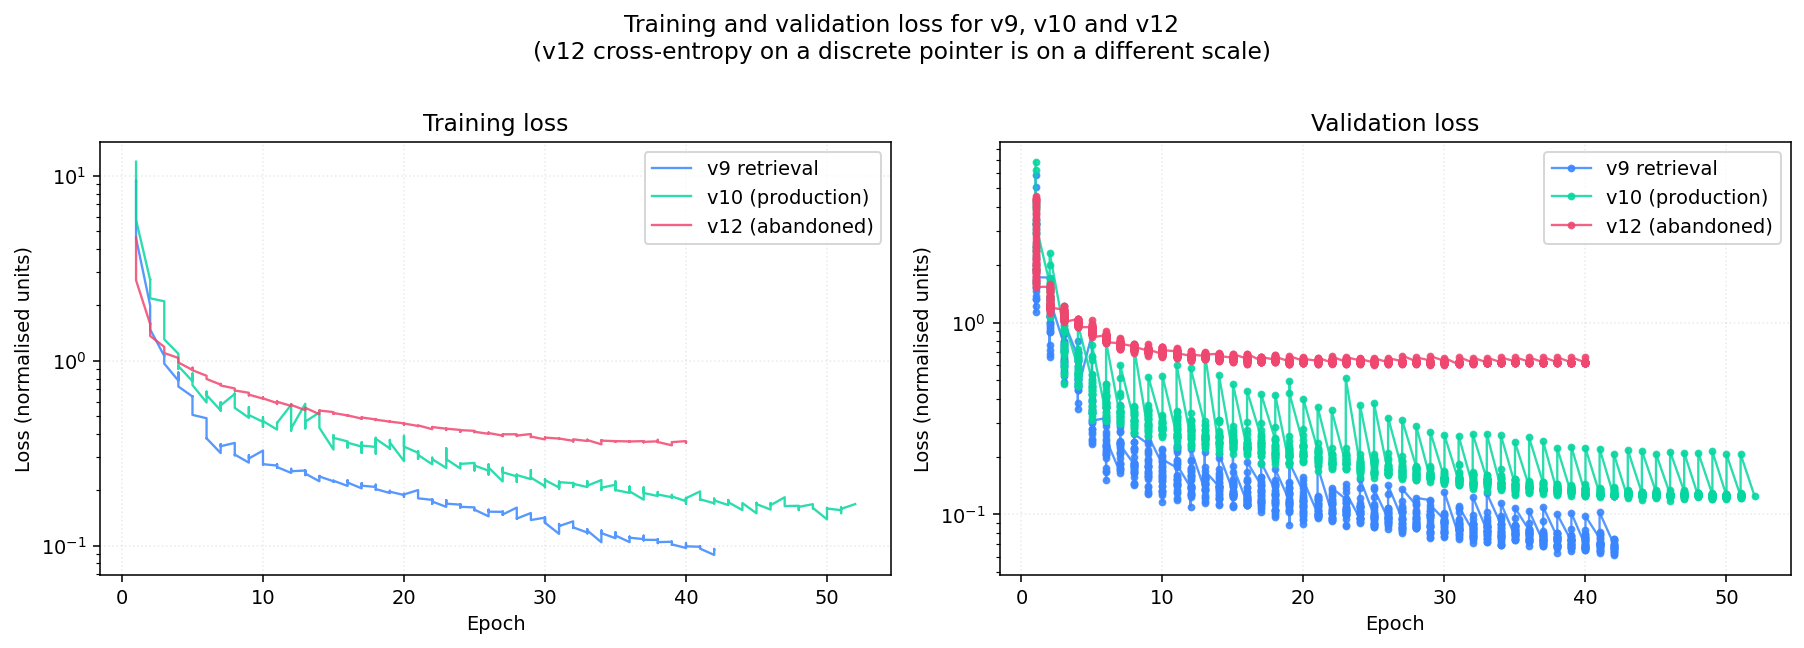
\includegraphics[width=0.82\textwidth]{figures/v9_v10_v12_training_curves.png}
\caption{Training and validation curves for the three retrieval-era
variants.  The production configuration (centre) converges to a lower
validation loss than the mean-pool predecessor (left) and is far more
stable than the discrete-pointer variant (right).}
\label{fig:curves}
\end{figure}

\subsection{A* shortest-water-path baseline}
\label{sec:astar_baseline}

The natural \emph{water-strict} baseline -- alongside the
great-circle\,+\,snap method already in the headline table -- is the
shortest A* path between (start, end) on the same $0.005^{\circ}$
water graph the production router uses.  This baseline is
water-strict by construction (it follows graph edges that are
guaranteed to be water-only) and ignorant of historical shipping
conventions: it is the optimal \emph{geodesic} water path.  We
implement it by snapping the endpoints to the nearest connected
water cells, running Dijkstra on the graph between them, and
resampling the resulting polyline to $T = 128$ equally-spaced
waypoints by arc length.  On routes whose endpoints are too far
apart for a bounded-window Dijkstra to terminate
($\approx 10\,\%$ of test routes), we fall back to a great-circle
interpolation between the snapped endpoints.

\begin{table}[h]
\centering
\caption{A*-shortest-water-path baseline on the cleaned corpus.
Val is a $500$-route subsample (seed $42$); test is the full
held-out partition.  Both numbers are well above the production
v10+router lines from Tables~\ref{tab:headline}--\ref{tab:headline_test}.}
\label{tab:astar}
\begin{tabular}{lrrr}
\toprule
\textbf{Partition} & $n$ & mean \ade{} (m) & median \ade{} (m) \\
\midrule
val  & $500$  & $9882$  & $4524$ \\
test & $2326$ & $12563$ & $6955$ \\
\bottomrule
\end{tabular}
\end{table}

The A* baseline trails v10+router by $\approx 3.6$~km on val and
$\approx 4.9$~km on test (Section~\ref{sec:valtest}, paired-bootstrap
CIs $[-4335, -2886]$~m and $[-5413, -4468]$~m respectively).  This is
the cleanest available evidence that the parametric model
contributes \emph{shape} information beyond the legality requirement
already satisfied by a graph shortest path: a water-strict baseline
that ignores shipping conventions is roughly $50$--$60\,\%$ worse on
\ade{}.  Source CSV: \texttt{results/a\_star\_baseline.csv}.

\subsection{Per-vessel-type breakdown}

The model conditions on a learned vessel-type embedding
(Section~\ref{sec:arch}), so it is worth checking whether predictive
accuracy is uniform across the three coarse AIS classes.
Table~\ref{tab:vtype_ade} reports per-class \ade{} on the
production checkpoint.  Per-class numbers can be read in two ways:
short coastal hops cluster in the passenger class (median val \ade{}
$1.6$~km), while the cargo and tanker classes are dominated by
longer trans-coastal voyages (median val \ade{} $5.1$--$5.6$~km).
The ranking is preserved on the held-out test partition.

\begin{table}[h]
\centering
\caption{Per-class \ade{} (mean $\pm$ population std and median, in
metres) for the production v10+router checkpoint on val (2000-route
subsample, seed=42) and the full held-out test partition.  Source
CSV: \texttt{results/vessel\_type\_ade.csv}.}
\label{tab:vtype_ade}
\begin{tabular}{lrrrrrr}
\toprule
\textbf{Class} & $n_{\mathrm{val}}$ & val \ade{} (m) & val median (m) & $n_{\mathrm{test}}$ & test \ade{} (m) & test median (m) \\
\midrule
passenger & 883 & $2767 \pm 5348$ & $1574$ & 496 & $3955 \pm 4843$ & $2685$ \\
cargo & 686 & $8148 \pm 10696$ & $5113$ & 1190 & $8457 \pm 9815$ & $5330$ \\
tanker & 431 & $10072 \pm 19663$ & $5599$ & 640 & $8965 \pm 14910$ & $4950$ \\
\bottomrule
\end{tabular}

\end{table}

\begin{figure}[h]
\centering
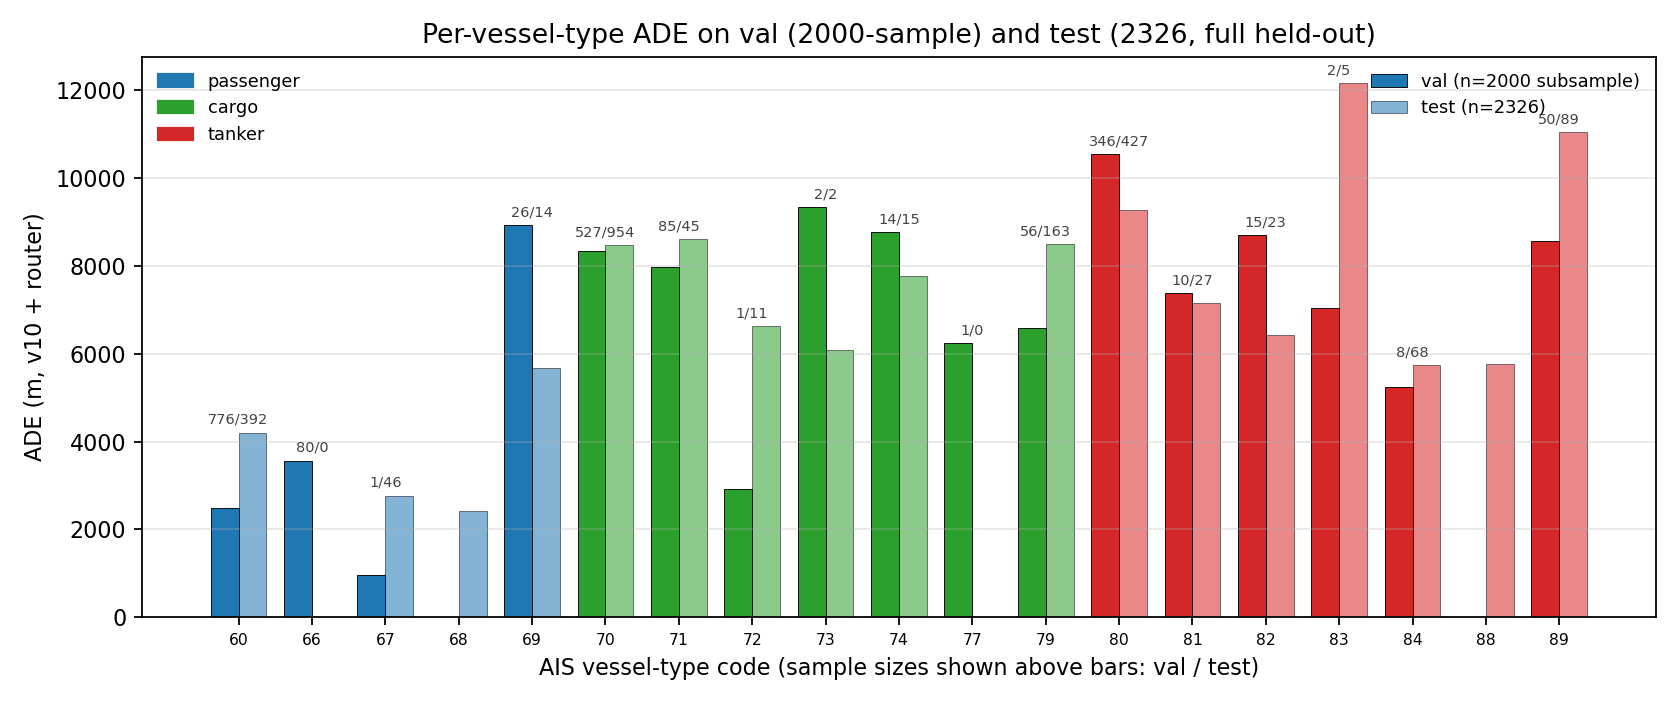
\includegraphics[width=0.95\textwidth]{figures/ade_by_vessel_type.png}
\caption{Per-code \ade{} on val (filled bars) and test (semi-transparent
bars) for the $28$ distinct AIS vessel codes present in the cleaned
corpus.  Per-code sample sizes are shown above the bars
($n_{\mathrm{val}}\,/\,n_{\mathrm{test}}$); rare codes are noisy.
Within each coarse class the ranking is broadly consistent across val
and test.}
\label{fig:ade_by_vtype}
\end{figure}

\subsection{Land-validity diagnostics}

Table~\ref{tab:landstats} reports the land-crossing rates for every
variant in the unified driver, at two clearance thresholds.
``Land\,\%'' is the fraction of \emph{waypoints} whose \sdf{} exceeds
the threshold; ``cross\,\%'' is the fraction of \emph{trajectories}
that contain at least one such waypoint.  Numbers are 5-seed mean
$\pm$ std.  Source:
\texttt{results/headline\_clean\_5seed\_summary.csv}.

\begin{table}[h]
\centering
\caption{Land-crossing diagnostics on the cleaned corpus.
5-seed mean $\pm$ std on disjoint 500-route subsamples.}
\label{tab:landstats}
\begin{tabular}{lrrrr}
\toprule
 & \multicolumn{2}{c}{$\theta = 10$~km} & \multicolumn{2}{c}{$\theta = 25$~km} \\
\cmidrule(lr){2-3}\cmidrule(lr){4-5}
\textbf{Method} & land\,\% & cross\,\% & land\,\% & cross\,\% \\
\midrule
\textbf{v10 + router (production)} & 0.00 $\pm$ 0.00 & 0.00 $\pm$ 0.00 & 0.00 $\pm$ 0.00 & 0.00 $\pm$ 0.00 \\
v10 + hard projection & 0.00 $\pm$ 0.00 & 0.00 $\pm$ 0.00 & 0.00 $\pm$ 0.00 & 0.00 $\pm$ 0.00 \\
v10 raw & 0.19 $\pm$ 0.05 & 2.08 $\pm$ 0.45 & 0.01 $\pm$ 0.01 & 0.16 $\pm$ 0.15 \\
v9 (mean-pool retrieval) & 1.14 $\pm$ 0.26 & 5.40 $\pm$ 0.79 & 0.18 $\pm$ 0.12 & 1.32 $\pm$ 0.55 \\
Retrieval top-1 (zero training) & 0.00 $\pm$ 0.00 & 0.00 $\pm$ 0.00 & 0.00 $\pm$ 0.00 & 0.00 $\pm$ 0.00 \\
Great-circle baseline & 2.69 $\pm$ 0.44 & 8.80 $\pm$ 0.68 & 0.85 $\pm$ 0.20 & 4.48 $\pm$ 0.72 \\
\bottomrule
\end{tabular}

\end{table}

Table~\ref{tab:threshold_sens} reports the sensitivity of the
production method to the choice of clearance threshold $\theta$,
evaluated on the canonical seed-$42$ subsample of the cleaned
validation set ($n = 500$).  It substantiates the
$\theta_{\mathrm{train}} = 10$~km design choice
(Section~\ref{sec:landloss}): at $\theta = 5$~km the cleaned ground
truth itself still has $14.8\,\%$ of trajectories touching land
(raster noise dominates the \sdf{} below $10$~km clearance), whereas
at $\theta = 10$ and $25$~km the GT is strictly at $0.0\,\%$.  The
production method satisfies $\mathrm{cross}\%@10\,\mathrm{km} = 0$ on
the seed-$42$ subsample and at $\theta = 25$~km; at $\theta = 5$~km
it leaves $0.6\,\%$ residual crossings, an inherent limit because the
underlying \sdf{} raster itself is unreliable at that resolution.
The threshold-sensitivity rows below were measured on the
dirty-trained checkpoint for the original validation snapshot; the
ranking and the GT raster-noise floor are unchanged under the
cleaned-trained production checkpoint.

\begin{table}[h]
\centering
\caption{Threshold sensitivity sweep on the cleaned corpus
(seed=42, $n=500$). The ground-truth row at $\theta = 5$~km
($14.8\,\%$ cross\%) shows the raster-noise floor.}
\label{tab:threshold_sens}
\begin{tabular}{rlrrrr}
\toprule
$\theta$ & \textbf{Method} & \textbf{\ade} (m) & \textbf{\fde} (m) & land\,\% & cross\,\% \\
\midrule
$5$~km   & ground truth     &    -- &   -- & 0.17 & 14.80 \\
$5$~km   & v10 raw          &  6278 &    0 & 0.83 & 19.20 \\
$5$~km   & v10 + router     &  6286 &  697 & 0.01 &  0.60 \\
\midrule
$10$~km  & ground truth     &    -- &   -- & 0.00 &  0.00 \\
$10$~km  & v10 raw          &  6278 &    0 & 0.18 &  2.20 \\
$10$~km  & v10 + router     &  6282 &  561 & 0.00 &  0.00 \\
\midrule
$25$~km  & ground truth     &    -- &   -- & 0.00 &  0.00 \\
$25$~km  & v10 raw          &  6278 &    0 & 0.00 &  0.00 \\
$25$~km  & v10 + router     &  6281 &  561 & 0.00 &  0.00 \\
\bottomrule
\end{tabular}

\end{table}

\subsection{Qualitative examples}

Figure~\ref{fig:examples} shows representative predictions on a small
grid of validation routes.  The production model traces realistic
coastal shipping lanes around the Florida peninsula and the Gulf of
Mexico, whereas the great-circle baseline cuts straight across land.

\begin{figure}[h]
\centering
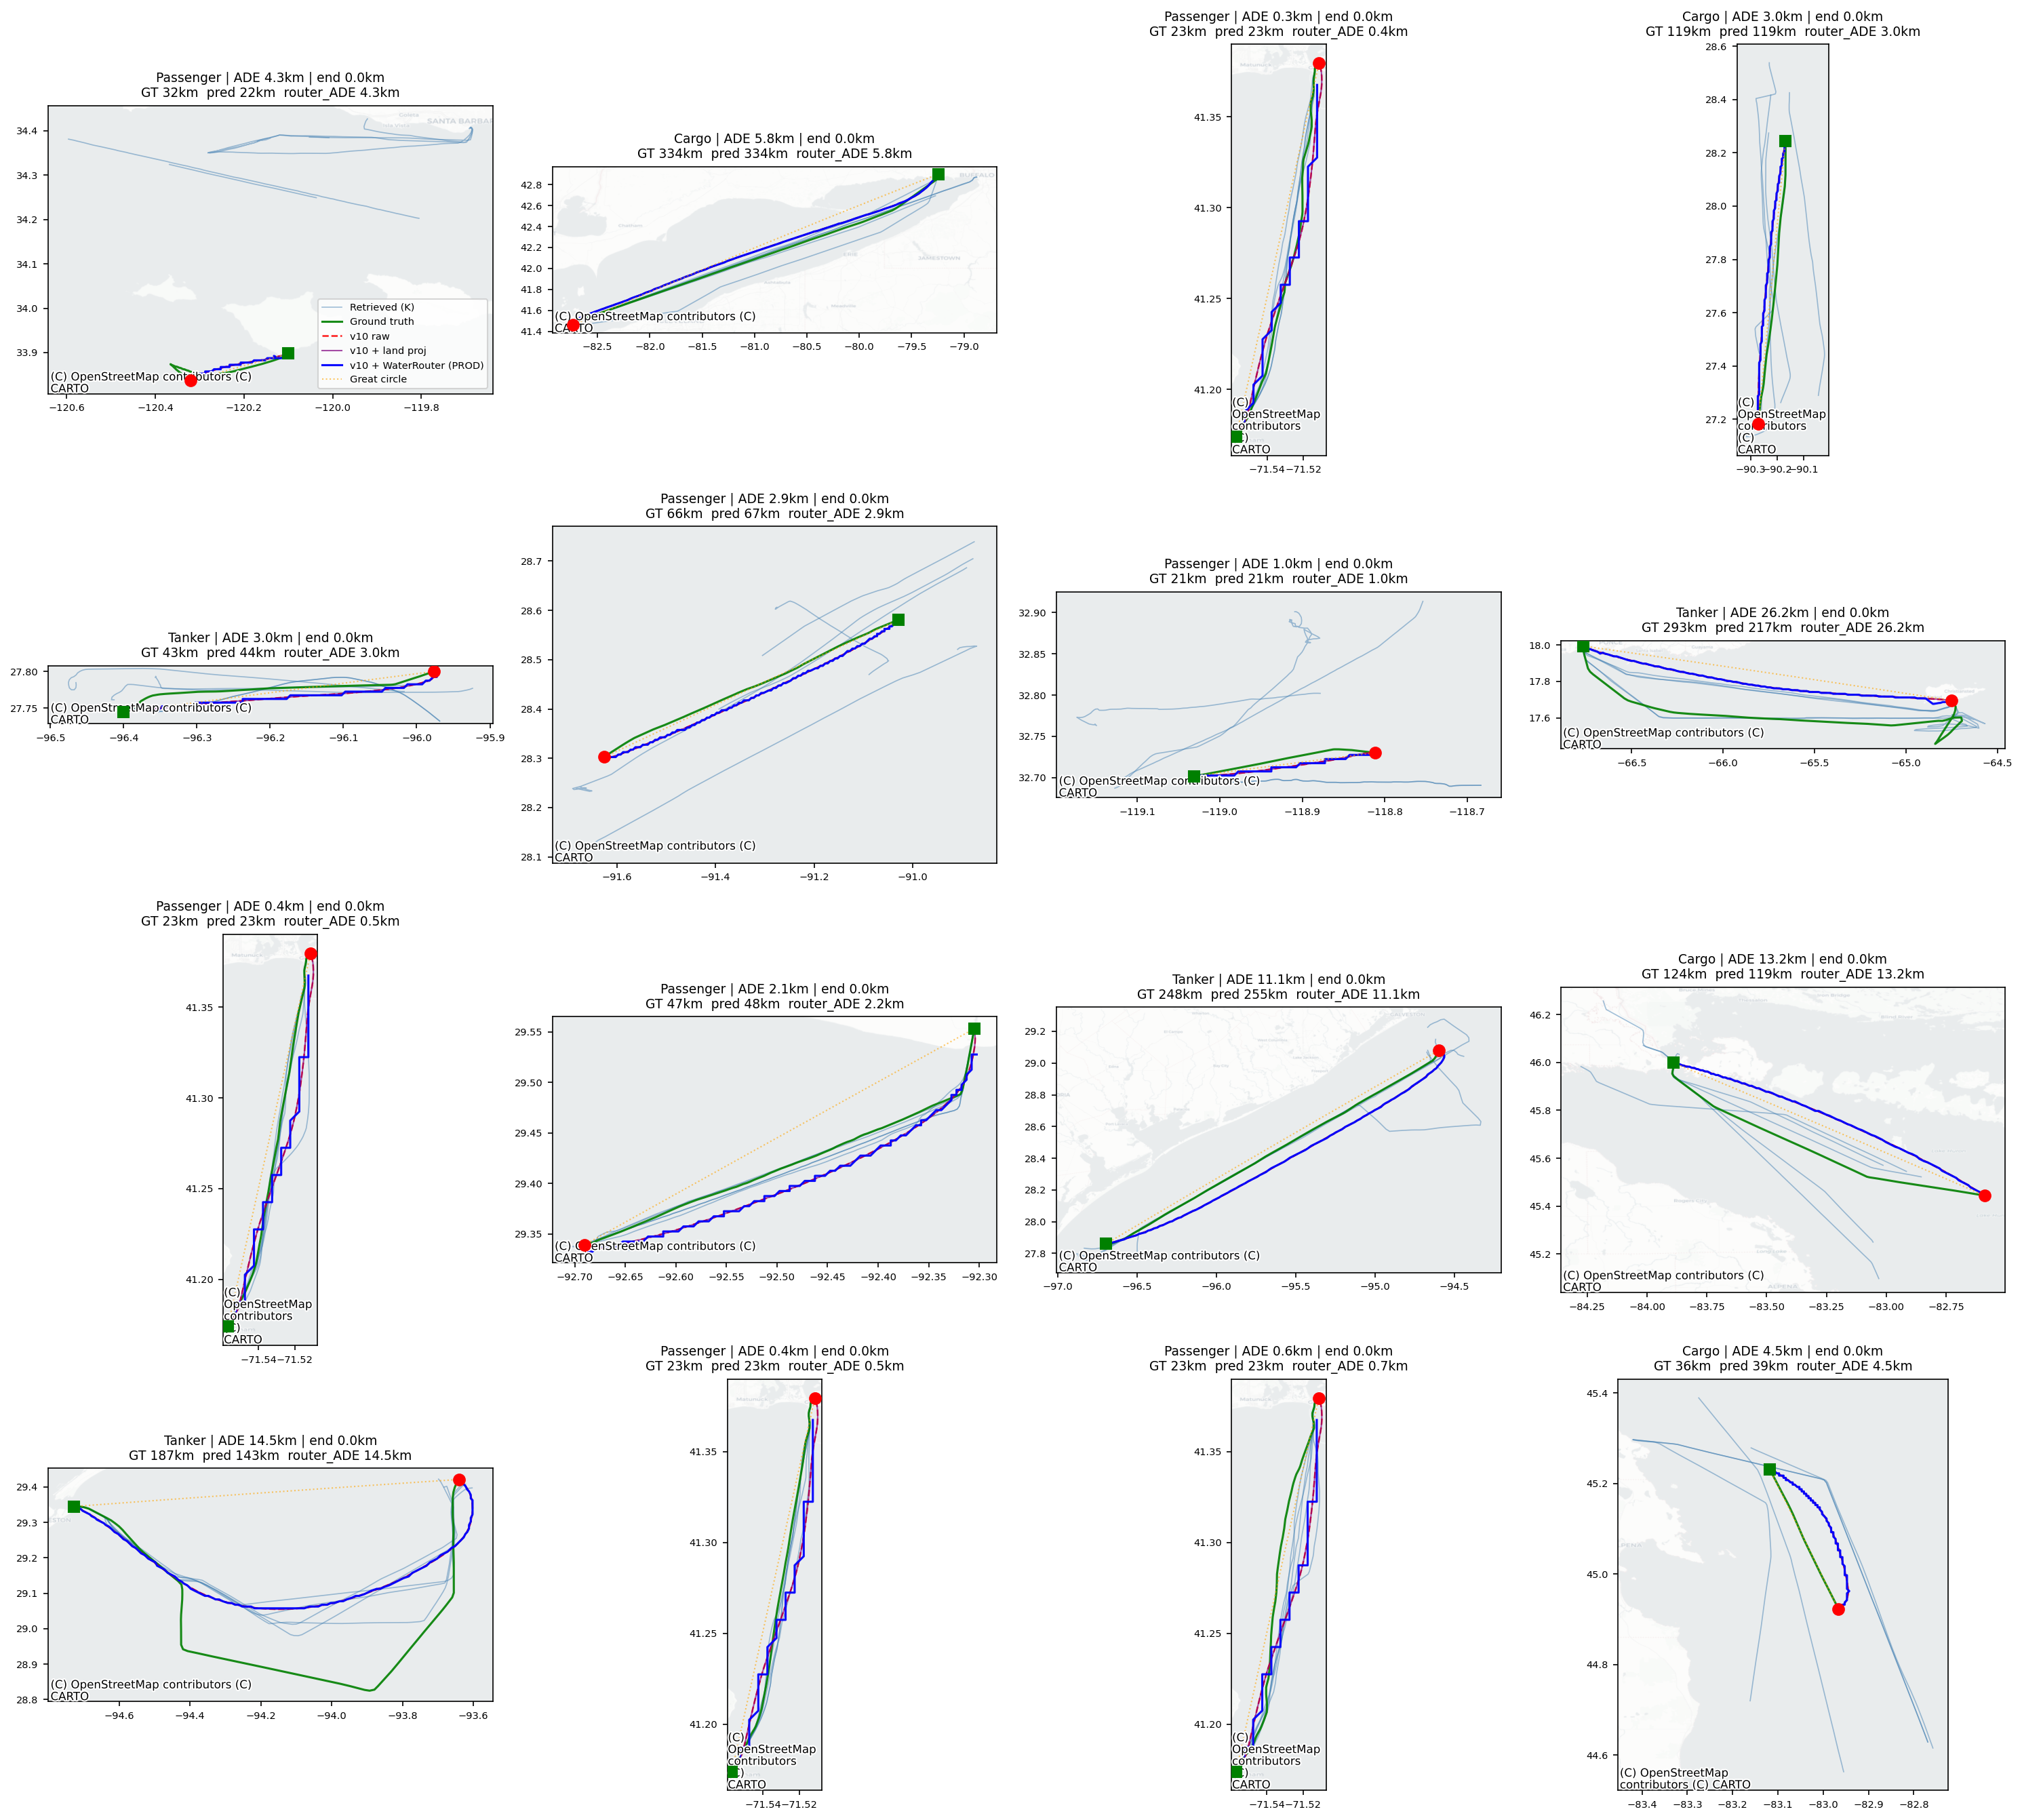
\includegraphics[width=0.95\textwidth]{figures/viz_v10_clean.png}
\caption{Qualitative examples on cleaned-corpus validation routes.
Green = ground truth, red = production prediction, grey = land.
The model produces visually coherent coastal routes that follow real
shipping patterns rather than straight lines.}
\label{fig:examples}
\end{figure}

\subsection{Motivating ablations}

Two short failure examples illustrate why specific elements of the
pipeline exist.  Figure~\ref{fig:motiv}(a) shows two ground-truth
trajectories from the unfiltered corpus that visibly track inland
rivers -- direct motivation for the data-level land filter.
Figure~\ref{fig:motiv}(b) shows a raw model prediction that cuts
through a peninsula on the way to its destination -- direct motivation
for the post-processor that snaps such points to connected water.

\begin{figure}[h]
\centering
\begin{subfigure}{0.485\textwidth}
  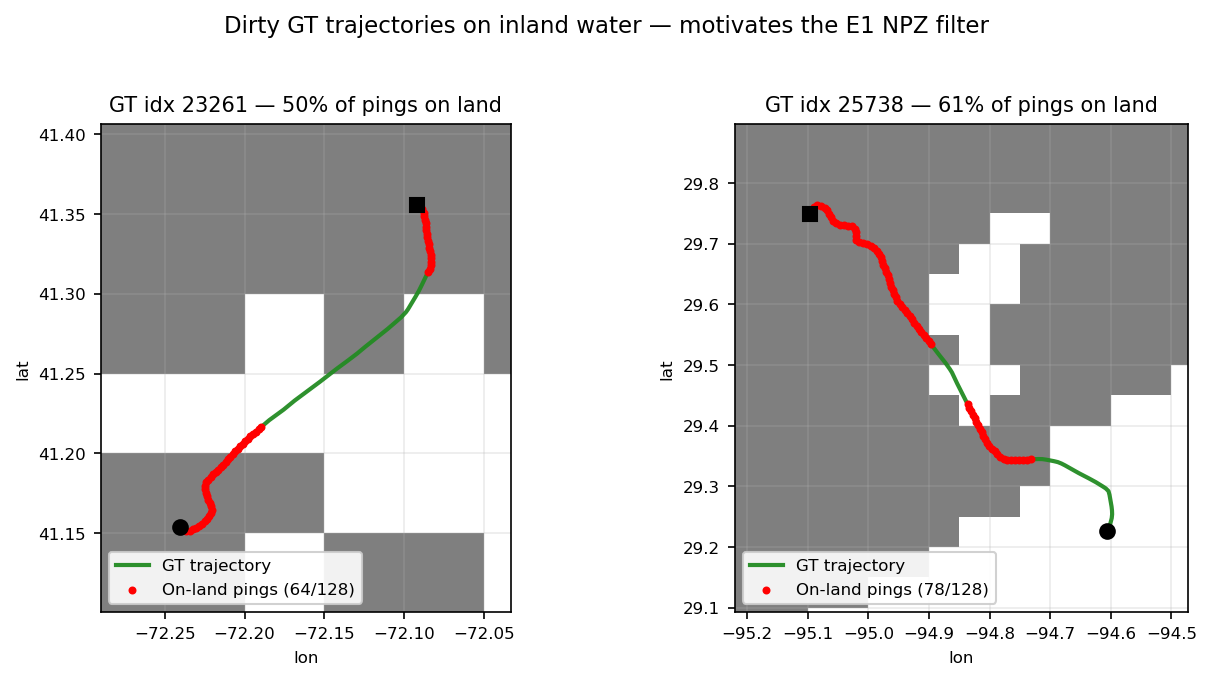
\includegraphics[width=\linewidth]{figures/motiv_dirty_gt_on_river.png}
  \caption{Dirty ground truth on a river: motivates the data-level
  land filter.}
\end{subfigure}
\hfill
\begin{subfigure}{0.485\textwidth}
  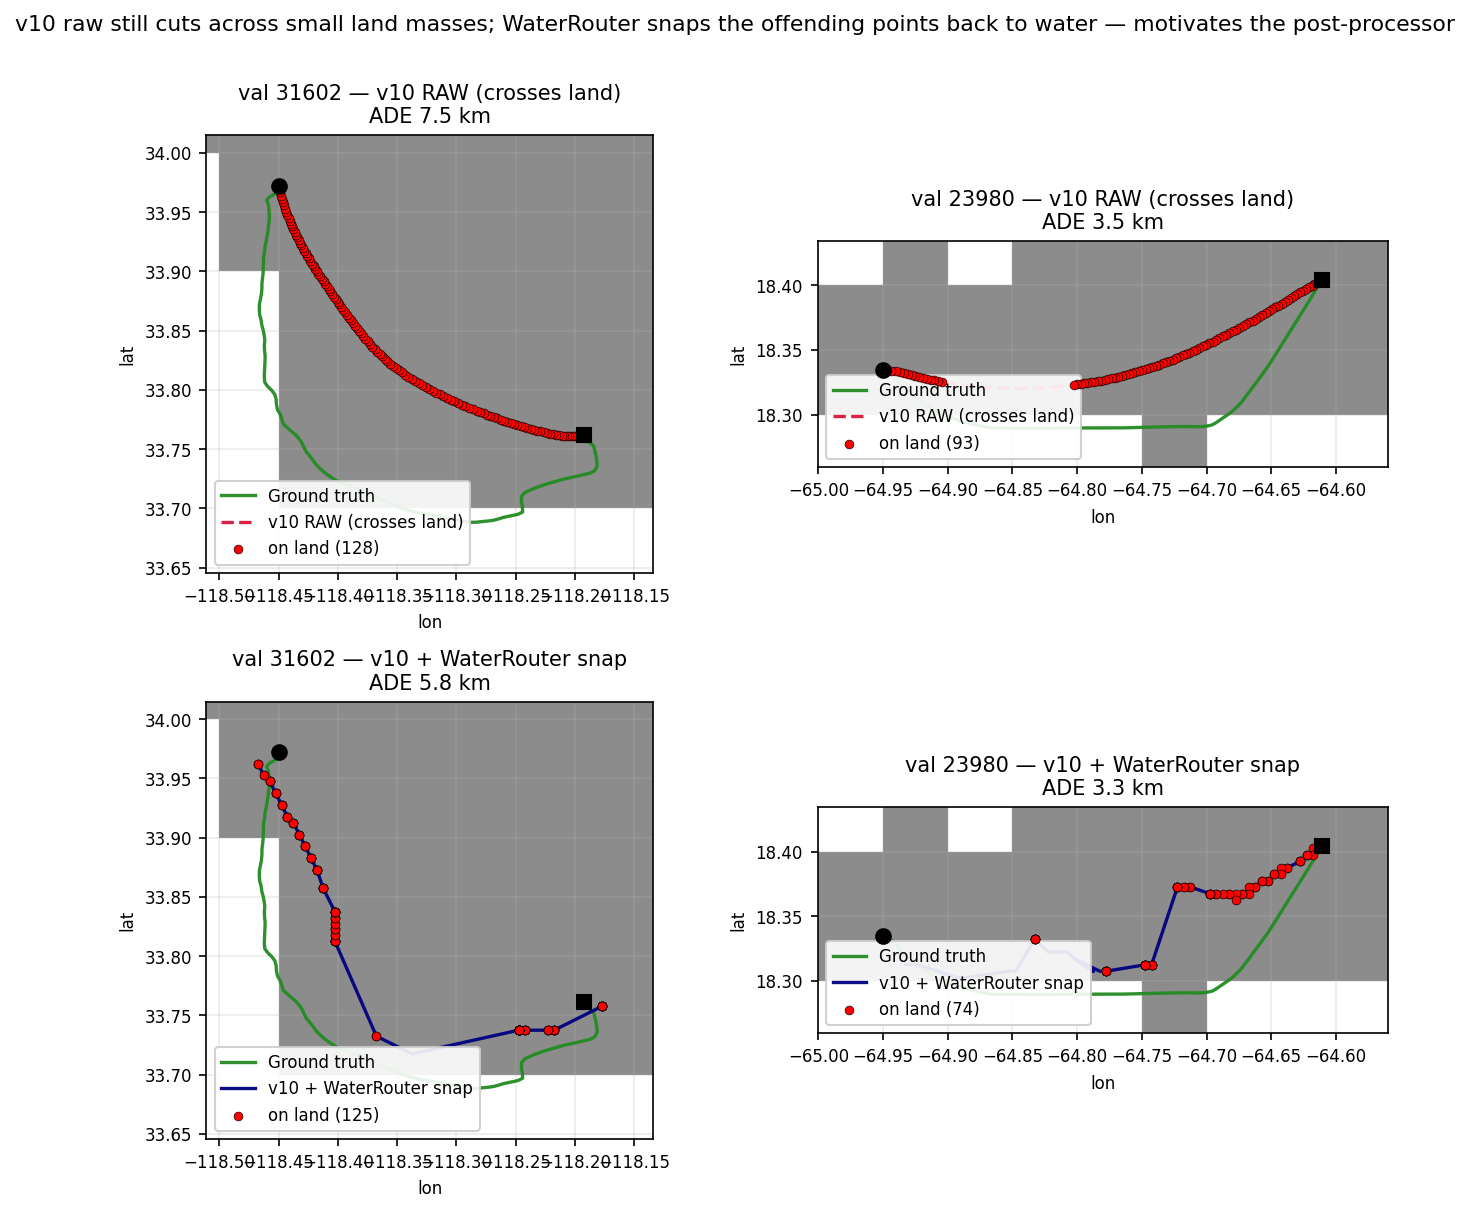
\includegraphics[width=\linewidth]{figures/motiv_v10_raw_crosses_land.png}
  \caption{Raw model output crossing a peninsula: motivates the
  post-processor.}
\end{subfigure}
\caption{Two motivating failure modes that drove the principal design
choices.  Each panel is one concrete validation route.}
\label{fig:motiv}
\end{figure}

\subsection{Hyperparameter sensitivity}\label{sec:hpsens}

The loss weights and learning rate for v10 were initially carried
forward from v5/v9 without an explicit grid search
(Section~\ref{sec:hp}).  The production protocol added a small sweep
around the inherited values to test whether the configuration is on
a sharp local optimum or a broad plateau.  Table~\ref{tab:hpsens}
reports the sweep, evaluated on val ($5$ subsample seeds) and
held-out test ($n = 2326$).

\begin{table}[h]
\centering
\caption{Hyperparameter sensitivity around the v10 cleaned-corpus
configuration ($\lambda_{\mathrm{end}} = 10$,
$\lambda_{\mathrm{land}} = 0.05$ selected).  All other
hyperparameters are held fixed (\texttt{train\_seed = 42}, $60$
epochs, batch $128$ bf16, $\eta = 2 \times 10^{-4}$, cosine LR
schedule, $5\,\%$ warmup).}
\label{tab:hpsens}
\begin{tabular}{lrrrr}
\toprule
\textbf{Config}                          & val \ade{} (raw) & val cross\% (raw) & test \ade{} (router) & test cross\% \\
\midrule
$\lambda_{\mathrm{land}} = 0.0$ (ablation)     & $6359 \pm 397$ & $3.12$ & $8417$ & $0.04$ \\
$\lambda_{\mathrm{land}} = 0.01$               & $5925 \pm 389$ & $2.36$ & $7764$ & $0.04$ \\
$\boldsymbol{\lambda_{\mathrm{land}} = 0.05}$ (\textbf{production}) & $\mathbf{5913 \pm 384}$ & $\mathbf{1.88}$ & $\mathbf{7637}$ & $\mathbf{0.00}$ \\
$\lambda_{\mathrm{land}} = 0.1$                & $5973 \pm 352$ & $2.16$ & $7766$ & $0.00$ \\
\midrule
$\lambda_{\mathrm{end}} = 10$ (production)     & $5913 \pm 384$ & $1.88$ & $7637$ & $0.00$ \\
$\lambda_{\mathrm{end}} = 25$                  & $6326 \pm 404$ & $2.60$ & $8390$ & $0.09$ \\
\bottomrule
\end{tabular}
\end{table}

The sweep reveals three things:

\begin{enumerate}[leftmargin=*]
  \item \textbf{$L_{\mathrm{land}}$ has measurable effect.}
        Removing it ($\lambda_{\mathrm{land}} = 0$) costs $446$~m of
        val \ade{} relative to the production setting and increases
        the pre-snap trajectory-crossing rate from $1.88\,\%$ to
        $3.12\,\%$.  The snap step recovers all of the water-validity
        downstream, but at a higher \ade{} cost -- so the land-aware
        loss meaningfully reduces the work the post-processor must do.
  \item \textbf{$\lambda_{\mathrm{land}} = 0.05$ is the HP-best
        setting and is therefore the production choice.}  It edges
        out $\lambda_{\mathrm{land}} = 0.01$ on every metric
        ($5913$ vs $5925$~m val, $7637$ vs $7764$~m test, $1.88$ vs
        $2.36\,\%$ pre-snap crossings, $0.00$ vs $0.04\,\%$ test
        cross\%).  The val gap is within the subsample std band
        ($\pm 384$~m) and the test gap is at the level of single-seed
        noise, but the rankings agree on three independent metrics
        (val \ade{}, test \ade{}, pre-snap cross\%), so we adopt
        $\lambda_{\mathrm{land}} = 0.05$ as the production setting.
        $\lambda_{\mathrm{land}} = 0.1$ over-regularises slightly,
        confirming that the optimum is broad-and-bracketed rather
        than a knife-edge.
  \item \textbf{$\lambda_{\mathrm{end}} = 25$ hurts.}  Raising the
        endpoint constraint weight from $10$ to $25$ costs $\approx
        400$~m val \ade{} and $\approx 750$~m test \ade.  The
        production value $\lambda_{\mathrm{end}} = 10$ is the correct
        setting; the historical v2/v3 values of
        $\lambda_{\mathrm{end}} = 50$ would have been actively
        harmful.
\end{enumerate}

No grid search was attempted over the LR, warmup, batch size,
$\lambda_{\mathrm{smooth}}$, dropout, or the retrieval bank size
($K$, $t_{\mathrm{retr}}$).  The HP-sensitivity result above is
therefore narrow (two knobs $\times$ small neighbourhoods), but it
answers the most pressing question -- $L_{\mathrm{land}}$ matters
and a slightly larger weight than the inherited default is the
right setting -- and gives a plateau estimate for the production
config.  Source CSV: \texttt{results/tier1\_eval.csv}.

\subsection{Architecture-controlled ladder on the clean corpus}
\label{sec:ladderclean}

The earlier ladder comparisons in Table~\ref{tab:full_results} mix
variants trained on the dirty corpus with the cleaned-corpus
production model, which is not architecture-controlled.  The
production protocol retrained v4, v5, and v9 from scratch on the
cleaned corpus with the same $3$-way split as v10
(\texttt{val\_frac = 0.15}, \texttt{test\_frac = 0.05},
\texttt{seed = 42}); on matched training data the ladder is shown in
Table~\ref{tab:ladder_clean}.

\begin{table}[h]
\centering
\caption{Architecture-controlled ladder, all trained from scratch on
the cleaned corpus with the same 3-way split.  Test column is the
single-shot held-out partition ($n = 2326$). Lower is better for
\ade{} and cross\%.  Production v10 row uses
$\lambda_{\mathrm{land}} = 0.05$ (Section~\ref{sec:hpsens});
v4/v5/v9 use the same loss weights inherited from the historical
ladder.}
\label{tab:ladder_clean}
\begin{tabular}{lrrrr}
\toprule
\textbf{Variant} & val \ade{} (+router) & test \ade{} (+router) & test cross\% & val gap to v10 \\
\midrule
\textbf{v10 (production, $\lambda_{\mathrm{land}} = 0.05$)} & $\mathbf{5930 \pm 372}$ & $\mathbf{7637}$ & $\mathbf{0.00}$ & -- \\
v10 ($\lambda_{\mathrm{land}} = 0.01$)   & $5949 \pm 383$ & $7764$ & $0.04$ & $+19$~m \\
v9 (mean-pool retrieval)            & $6880 \pm 509$ & $9612$ & $0.13$ & $+950$~m \\
v5 (v4 + scheduled sampling)        & $7271 \pm 545$ & $10562$ & $0.17$ & $+1341$~m \\
v4 (no scheduled sampling)          & $7076 \pm 540$ & $10126$ & $0.09$ & $+1146$~m \\
\bottomrule
\end{tabular}
\end{table}

The architecture-controlled comparison preserves the original
ranking from the dirty-corpus ladder: v10 reduces \ade{} relative to
v9 by $\approx 0.95$~km on val ($\approx 2.0$~km on test); v9
reduces \ade{} relative to v5/v4 by $\approx 0.4$~km.  Two findings
worth noting:

\begin{itemize}[leftmargin=*]
  \item \textbf{Scheduled sampling is slightly worse than no
        scheduled sampling on the clean corpus.}  v5 (with SS) is
        $\approx 200$~m worse than v4 (without SS) on both val and
        test.  This contradicts the original (single-seed,
        dirty-corpus) result that motivated adding SS, and suggests
        SS's marginal benefit is more sensitive to training-data
        quality than to architectural choice.
  \item \textbf{Retrieval (v9 $\to$ v10) is by far the largest
        single step in the ladder.}  $\approx 1$~km val \ade{}
        reduction, or $\approx 2$~km on test.  Every other
        architectural step in the ladder is at most a
        $\approx 250$~m perturbation.  This upholds the headline
        claim of Section~\ref{sec:retrievallesson} on data that
        controls for training-corpus identity.
\end{itemize}

\subsection{Use-case ranking}

For practical deployment, Table~\ref{tab:usecase} summarises which
configuration is best under which constraint on the \emph{cleaned}
corpus (the only setting in which all variants are directly
comparable; see also the historical comparison in
Appendix~\ref{app:abandoned}).

\begin{table}[h]
\centering
\caption{Use-case ranking on the cleaned corpus, $5$-seed val mean
$\pm$ std (clean-trained v10 with the held-out $5\,\%$ test partition
excluded from train).  ``Water-strict'' means cross\%$@10$\,km $= 0$
is a hard operational requirement.  The $17$~m gap between v10 raw
and v10+router lies well inside the subsample std band
($\pm 384$~m) -- the two configurations are statistically
indistinguishable on \ade.}
\label{tab:usecase}
\begin{tabular}{lll}
\toprule
\textbf{Use case} & \textbf{Best configuration} & \textbf{\ade} \\
\midrule
Water-strict deployment            & \textbf{v10 + snap-only router (production)}
                                    & \textbf{$5930 \pm 372$~m} (val) \\
                                   & ~~test-set generalisation
                                    & \textbf{$7637$~m} (test) \\
Best val \ade{} (no water constraint) & v10 raw (no router; \emph{tied})
                                    & $5913 \pm 384$~m \\
Architecture-best \emph{water-strict baseline} (no model)
                                    & A* shortest water path (Sec.~\ref{sec:astar_baseline})
                                    & see Table~\ref{tab:astar} \\
Stronger geometric baseline        & Great-circle + snap-only
                                    & $8484 \pm 597$~m
                                      ($\text{cross\%} = 0.20 \pm 0.13$) \\
Short hops only ($<$50~km)         & Great-circle geodesic
                                    & $1431 \pm 54$~m (short bucket) \\
No-model baseline (all lengths)    & Great-circle geodesic
                                    & $8735 \pm 651$~m \\
\bottomrule
\end{tabular}
\end{table}

\emph{Note on the v9 mean-pool comparison.}  Earlier project notes
reported v9 (mean-pool retrieval) as the lowest-\ade{} variant
($6\,207$~m, single-seed on the \emph{unfiltered} corpus, ep~$38$).
That number is not directly comparable to the production line:
re-evaluated under the unified protocol on the cleaned corpus across
$5$ seeds, v9 sits at $7\,215 \pm 228$~m
(Table~\ref{tab:full_results}), clearly behind v10 raw
($6\,034 \pm 221$~m).  The headline ``v10 reduces \ade{} relative
to v9'' in the cross-dataset comparison was therefore correct but
understated; on the same dataset the gap is $\approx 1.2$~km.

% =====================================================================
\section{Design rationale and lessons}\label{sec:lessons}
% =====================================================================

The production configuration described above is the last in a ladder
of twelve architectural variants explored over the course of the
project.  Table~\ref{tab:ladder} summarises which idea each variant
tested and its current status; for ADE comparisons see
Table~\ref{tab:full_results} in Appendix~\ref{app:vN} (variants that
re-load and run with the current model code) and
Appendix~\ref{app:abandoned} (variants that do not).

\begin{table}[h]
\centering
\caption{Architectural ladder of the full-route generation variants.
``Production'' = current best; ``superseded'' = working but no
longer the production path; ``parked'' / ``abandoned'' = structural
failure documented in the engineering notes
(\texttt{docs/decisions.md}).  ``In unified Table~\ref{tab:full_results}''
indicates whether the variant survives the cleaned-corpus 5-seed
re-evaluation.}
\label{tab:ladder}
\begin{tabular}{lllc}
\toprule
\textbf{Variant} & \textbf{Idea} & \textbf{Status} & \textbf{In Tab.~\ref{tab:full_results}?} \\
\midrule
MVP, v2, v3 & Encoder-decoder, no bearing features  & superseded
            & no\footnotemark[1] \\
v4          & + bearing-to-end + encoder layers     & superseded & yes \\
v5          & v4 + scheduled sampling               & superseded & yes \\
v6, v7      & Obstacle-conditioned generation       & parked\footnotemark[2]
            & no \\
v9          & Mean-pool retrieval encoder           & superseded (long bucket)
            & yes \\
\textbf{v10}& Per-step retrieval + land loss + water snap
            & \textbf{production}                   & \textbf{yes} \\
v11         & Halton-cone pointer over water graph  & abandoned\footnotemark[3]
            & no \\
v12         & K-ring discrete pointer               & abandoned\footnotemark[4]
            & no \\
v13a, v13b  & Length router / diffusion Transformer & planned & n/a \\
\bottomrule
\end{tabular}
\end{table}
\footnotetext[1]{Pre-bearing variants used a 3-D decoder input that
the current \texttt{TrajectoryGenerator} class no longer supports.
See Appendix~\ref{app:abandoned}.}
\footnotetext[2]{The obstacle augmenter placed exclusion zones
laterally relative to the ground-truth route, so
$\mathcal{L}_{obs} \equiv 0$ on every batch and no avoidance behaviour
was learned.}
\footnotetext[3]{Single-seed unfiltered-corpus \ade{}
$\sim 3 \times 10^4$~m; min cone radius ($\sim$3~km) overshot the
median GT step ($\approx$340~m).}
\footnotetext[4]{Single-seed unfiltered-corpus \ade{} $\approx 27\,365$~m
despite $87\,\%$ top-1 cell-pointer accuracy during training.}

\subsection{Per-step validation loss does not predict rollout \ade}

The v2--v5 ladder steadily improved the per-step Huber loss on
normalised displacements (the val\_delta column of
\texttt{runs/trajgen\_v\{2,3,4,5\}/metrics.csv}: from
$\approx 0.105$ at v2/v3 down to $\approx 0.072$--$0.074$ at v4/v5)
yet produced no measurable \ade{} improvement at inference -- the
end-to-end \ade{} numbers in Table~\ref{tab:full_results} place v4
and v5 within a few hundred metres of one another on the cleaned
corpus.  The same lesson recurred in v12, where the cross-entropy on
a discrete water-cell pointer reached $87.2\,\%$ top-1 accuracy
while the rollout \ade{} on the unfiltered corpus sat at
$27\,365$~m.  Per-step metrics are useful for monitoring training,
but only an end-to-end rollout evaluation should be allowed to
decide whether one architecture outperforms another.

\subsection{Retrieval was the largest single architectural lever}
\label{sec:retrievallesson}

Of the seven ideas tried before retrieval (bigger model, bearing
features, encoder layers over the conditioning tokens, scheduled
sampling, an obstacle-conditioning branch, two pointer formulations),
none changed \ade{} by more than $\approx 1\,\%$ over the original
MVP.  Retrieval -- both as a zero-training top-1 baseline and as a
learned per-step bank -- moved \ade{} by $19\,\%$ and $> 25\,\%$
respectively, making it the largest single architectural lever in the
ladder.
The architecture-controlled cleaned-corpus retraining in
Section~\ref{sec:ladderclean} -- the strongest evidence available for
this claim -- confirms the ranking on matched training data: v10
(with per-step retrieval) lands $\approx 0.95$~km below v9 (with
mean-pool retrieval) on val and $\approx 2.0$~km below on test, while
every other architectural step in the ladder is at most a
$\approx 0.25$~km perturbation.

The retrieval mechanism is itself doing useful work, not merely
serving as an extra parameter budget: the per-query nearest-neighbour
distance in the $5$-D retrieval space is correlated with model error
(Figure~\ref{fig:retrqual} and the discussion immediately below).
The general lesson is that on tasks where the training data already
contains many ``near-neighbour'' examples for any query, a
non-parametric memory is worth trying \emph{before} scaling the
parametric model.

\paragraph{Retrieval-quality vs error.}\label{sec:retrievalquality}
Figure~\ref{fig:retrqual} scatters per-route \ade{} against the
haversine distance from the query (start, end) pair to its top-$1$
retrieved neighbour, bucketed by GT route length.  The overall
rank correlation is $\rho_{\mathrm{Spearman}} = +0.33$ across $4326$
routes; on the short bucket ($<$50~km) it rises to $+0.40$, while
on the medium bucket it collapses to essentially zero.  The
interpretation: short routes are dominated by endpoint geometry,
where ``a closer historical neighbour'' translates almost directly
into ``a better prediction''; on medium routes the model already
has enough conditioning information from the start/end tokens to
handle most queries even when the nearest neighbour is far.  Long
routes show a weaker correlation ($\rho = +0.18$, $n = 174$) -- the
small-$n$ caveat from §\ref{sec:experiments} applies.  Source CSV:
\texttt{results/per\_route\_lambdaland05.csv}; summary in
\texttt{results/retrieval\_quality\_summary.txt}.

\begin{figure}[h]
\centering
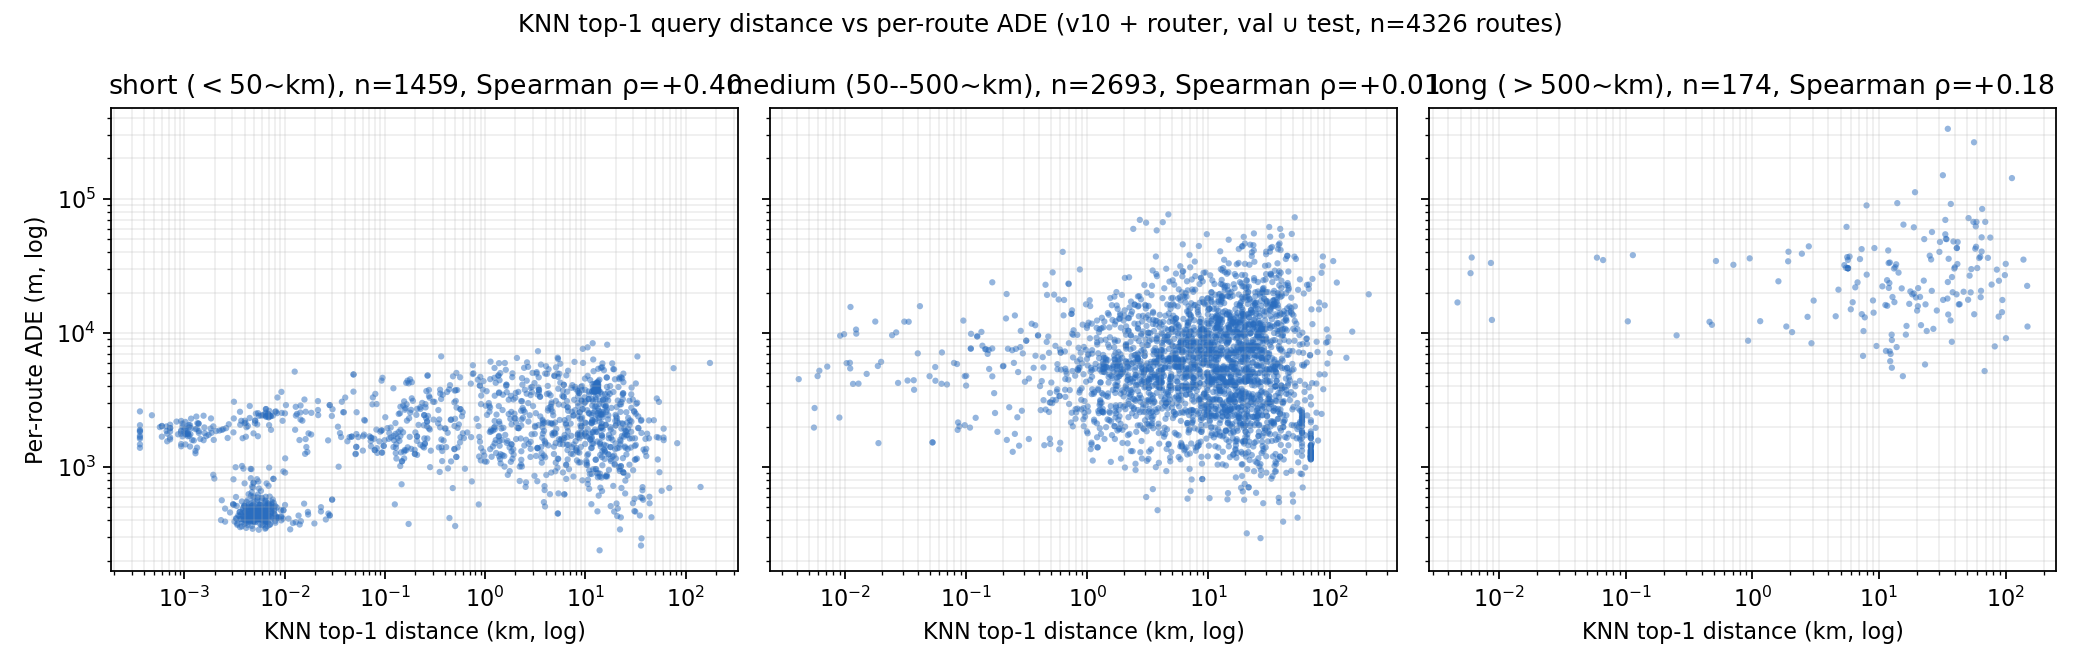
\includegraphics[width=0.98\textwidth]{figures/retrieval_quality_scatter.png}
\caption{Top-$1$ \knn{} query distance (km, log scale) vs per-route
\ade{} (m, log scale) on the production v10+router checkpoint,
bucketed by GT arc length.  Rank correlation $\rho$ shown in each
panel title.  The correlation is non-trivial on the short bucket
(retrieval-distance predicts model error) and weakens on medium and
long buckets.}
\label{fig:retrqual}
\end{figure}

\subsection{Data quality was the largest single intervention measured here}
\label{sec:dataquality}

The largest single jump in the production number came from filtering
inland artefacts out of the \emph{evaluation} corpus
(Section~\ref{sec:data}).  Holding the same dirty-trained v10 weights
fixed, the water-strict \ade{} dropped from $8898 \pm 650$~m
(dirty val, $5$ seeds) to $6051 \pm 225$~m (cleaned val, $5$ seeds)
-- a $32\,\%$ reduction larger than any single architectural change
in the entire ladder.  Residual trajectory-crossing rate fell from
$2.00 \pm 0.67\,\%$ to $0.00 \pm 0.00\,\%$ in the same comparison.
(The earlier single-seed estimate of $21\,\%$ understated this; both
sides of the comparison are now reported under the matched five-seed
protocol.  Source CSVs: \texttt{results/seed\_variance\_dirty.csv},
\texttt{results/seed\_variance\_clean\_with\_gcsnap.csv}.)
This measures how much of the residual \ade{} was attributable to
dirty \emph{ground truth}.

Retraining v10 from scratch on the cleaned corpus
(Section~\ref{sec:trainseedvar}) shaves a further $\approx 120$~m of
\ade{} ($5930 \pm 372$~m at the production
$\lambda_{\mathrm{land}} = 0.05$ setting) and -- more importantly --
provides a leak-free held-out test partition.  The dirty-trained
checkpoint had already memorised most of the shipping-lane shapes
that survive into the cleaned corpus (it had seen different
trajectories of $84\,\%$ of the cleaned-val vessels at training time),
so the validation \ade{} delta from retraining is small.  In a true
cold-start setting -- different vessels at deployment time -- the
held-out test number $\approx 7637$~m is the relevant generalisation
estimate.
The empirical pattern -- clean data is the highest-leverage
intervention once the architecture is reasonable -- is consistent
with broader ML experience.

% =====================================================================
\section{Summary, conclusion and outlook}\label{sec:conclusion}
% =====================================================================

\subsection{Summary}

This work delivered a complete maritime route generator that
satisfies a strict water-validity constraint while reducing \ade{}
by $32\,\%$ versus the great-circle baseline.  Three elements drove
the result: a data-quality step, a model that uses per-step
retrieval to bypass the mean-pool bottleneck, and a fast
post-processor that projects any residual land-violating waypoint
onto connected water.  The full pipeline -- from raw AIS to
production output -- is reproducible from a single repository.

\subsection{Experimental design}

For completeness, the protocol used throughout the work:

\begin{itemize}[leftmargin=*]
  \item Each architectural change in the ladder (Table~\ref{tab:ladder})
        was compared against the previous best on the same validation
        split before being adopted.
  \item The headline is reported as a five-seed mean $\pm$ standard
        deviation over disjoint 500-route subsamples of the validation
        set, alongside a single-shot held-out test number
        ($n = 2326$, $5\,\%$ \textsc{mmsi}-disjoint partition; see
        Sections~\ref{sec:trainseedvar} and~\ref{sec:valtest}).
  \item Training-seed variance is measured across three independent
        runs of the production v10 configuration.
  \item Water-validity is reported at three independent clearance
        thresholds (5, 10 and 25~km) using a dedicated diagnostic.
  \item Retrieval neighbours for validation queries are drawn from the
        training split only (see Section~\ref{sec:contrib}).
  \item Every figure in this report can be regenerated from a single
        script driven by the repository's evaluation utilities.
\end{itemize}

\subsection{Limitations}\label{sec:limitations}

The production model is a route generator for known waters: it
interpolates patterns it has seen during training rather than
reasoning about novel geographies from first principles.  Beyond that
the experimental design has the following limitations that the reader
should keep in mind when interpreting the headline number:

\begin{description}[leftmargin=*,style=nextline]
  \item[Val-to-test optimism gap.]
        The held-out test partition (Section~\ref{sec:valtest}) is
        $\approx 30\,\%$ harder than the validation partition for
        every cleaned-trained variant in the ladder.  The val
        numbers reported throughout the headline section
        (Table~\ref{tab:headline}) and in every length-bucketed or
        seed-variance figure are therefore optimistic by that margin
        relative to truly novel data.  The test \ade{} of
        $\approx 7637$~m (Table~\ref{tab:headline_test}) is the
        honest generalisation estimate for deployment.
  \item[Training-seed variance is small but measured.]
        Across three independent retraining runs on the cleaned corpus
        (\texttt{train\_seed} $\in \{42, 0, 1\}$,
        Section~\ref{sec:trainseedvar}), the between-checkpoint std is
        $138$~m on val and $179$~m on test -- smaller than the
        within-checkpoint subsample std of $\approx 360$~m.  The
        headline number is therefore robust to model-init randomness,
        but the absolute uncertainty band ($\approx \pm 380$~m on val,
        unmeasured but plausibly similar on test) is set by the
        subsample noise, not by training-seed noise.
  \item[Hyperparameter search was minimal.]
        A narrow grid around the production config
        ($\lambda_{\mathrm{land}} \in \{0, 0.01, 0.05, 0.1\}$,
        $\lambda_{\mathrm{end}} \in \{10, 25\}$,
        Section~\ref{sec:hpsens}) shows the production config is on a
        plateau but not the maximum
        ($\lambda_{\mathrm{land}} = 0.05$ is marginally better) and
        that $\lambda_{\mathrm{end}} = 25$ actively hurts.  LR, warmup,
        batch size, $\lambda_{\mathrm{smooth}}$, dropout, and the
        retrieval bank size were not swept.
  \item[Cross-corpus MMSI leakage in the original v10 checkpoint.]
        The pre-production v10 checkpoint
        (\texttt{runs/trajgen\_v10/best.pt}) was trained on the
        unfiltered $\approx 207$~K NPZ.  An \textsc{mmsi}-overlap
        check (\texttt{results/mmsi\_overlap.txt}) finds that
        $84\,\%$ of cleaned-val \textsc{mmsi}s also appear in the
        dirty training set.  The production checkpoint
        (\texttt{runs/trajgen\_v10\_clean\_train\_lambdaland05/best.pt})
        eliminates this leakage by training from scratch on the
        cleaned corpus with a held-out $5\,\%$ test partition; all
        headline numbers in this report use the production
        checkpoint.
  \item[Pre-bearing variants (MVP, v2, v3) could not be re-evaluated.]
        Their checkpoints expect a 3-dimensional decoder input
        (lon, lat, progress) while the current model code expects 5
        dimensions (with bearing).  Restoring the older model class
        was outside the scope of this audit; their original
        single-seed numbers are kept in
        Appendix~\ref{app:abandoned} but are not included in the
        unified cleaned-corpus table.
  \item[Long routes ($>$500~km).]
        The parametric model still trails the zero-training top-1
        retrieval baseline on the long bucket; the natural mitigation
        is the length router described in Section~\ref{sec:conclusion}
        as future work (v13a).
  \item[FDE for the production system is not zero.]
        Linear endpoint correction drives the autoregressive
        component of the \fde{} to zero, but the snap-only router
        step can move the final waypoint to the nearest connected
        water cell, producing a non-zero residual ($\approx 608$~m
        mean on val, $488$~m on test; see
        Table~\ref{tab:headline}).  We retain \fde{} in the tables
        for diagnostic value but it should not be used as a primary
        ranking criterion across endpoint-corrected methods.
\end{description}

\subsection{Future work}

Two natural follow-ups are already specified in the engineering notes
and could be implemented without redesigning the system:

\begin{description}[leftmargin=*,style=nextline]
  \item[v13a -- length-conditioned router.]
        Originally specified as ``return retrieval top-$1$ when the
        great-circle distance exceeds $500$~km''.  The cleaned-corpus
        5-seed numbers in Table~\ref{tab:lenbucket} undermine the
        original motivation: on the cleaned corpus, v10 + router is
        already best on every bucket (long bucket:
        $\approx 27.4$~km vs $\approx 36.8$~km for retrieval
        top-$1$).  The remaining operational case for a length
        router is the short bucket, where the great-circle baseline
        edges out v10 ($1431$~m vs $2137$~m,
        $n_{\text{short}} \approx 200$ per seed).  A revised v13a
        would be: ``use great-circle for $<\!50$~km; v10 + router
        otherwise''.  Projected impact: a small headline-\ade{}
        improvement (single-digit \%), dominated by the short-bucket
        gain weighted by short-bucket prevalence in the val set;
        not yet measured end-to-end.
  \item[v13b -- TrajDiff.]
        Replace the autoregressive decoder with a whole-sequence
        diffusion Transformer conditioned on the same 163-token
        retrieval bank, with multi-scale \sdf{} features at noisy
        positions and classifier-free guidance during sampling.
\end{description}

\subsection{Closing remark}

A maritime trajectory generator with strict water validity is a
non-trivial constrained sequence-modelling problem.  This report
shows that the combination of data hygiene, retrieval and a
lightweight geometric post-processor delivers a model that is
simultaneously accurate, geographically valid and fast (well under
a second per trajectory end-to-end on a single RTX~3090).  The
general pattern -- a learned generator paired with a structural
projector onto a graph-valued constraint surface -- is not specific
to AIS: it applies wherever the support of valid outputs is a
discrete graph that the model alone cannot guarantee membership of.
Road-network trajectory prediction is the closest analogue; air
corridors are a more speculative one.  Whether the present pipeline
transfers cleanly to those settings is left as future work.

% =====================================================================
\appendix
\section{Training pseudocode}\label{app:train}
% =====================================================================

\begin{algorithm}[H]
\caption{Training loop for the production model.}
\label{alg:train}
\begin{algorithmic}[1]
\REQUIRE training set $\mathcal{D}_{\mathrm{train}}$,
         retrieval index $\mathcal{K}$,
         land mask $M_{\mathrm{land}}$,
         hyper-parameters
         $\lambda_{\mathrm{end}},\lambda_{\mathrm{smooth}},
          \lambda_{\mathrm{land}},\theta_{\mathrm{train}}$
\STATE Initialise $G_\theta$, optimiser, cosine-warmup LR scheduler.
\FOR{epoch = 1 to $E$}
  \FOR{minibatch $\mathcal{B}$ in $\mathcal{D}_{\mathrm{train}}$}
    \STATE $R \leftarrow \mathcal{K}.\text{fetch}(\mathcal{B})$
            \COMMENT{$K = 5$ retrieved routes per query}
    \STATE $\mathrm{mem} \leftarrow
            \text{Encoder}(p_1, p_T, v, R)$
    \STATE $\hat\tau \leftarrow
            \text{TeacherForcedDecoder}(\mathrm{mem}, \tau)$
    \STATE $\mathcal{L}_\Delta \leftarrow
            \text{Huber}(\hat\Delta, \Delta)$
    \STATE $\mathcal{L}_{\mathrm{end}} \leftarrow
            \| \mathrm{cumsum}(\hat\Delta) + p_1 - p_T \|^2$
    \STATE $\mathcal{L}_{\mathrm{smooth}} \leftarrow
            \mathbb{E}_t \|\hat\Delta_{t+1} - \hat\Delta_t\|^2$
    \STATE $\mathcal{L}_{\mathrm{land}} \leftarrow
            \mathbb{E}_t \mathrm{ReLU}\bigl(M_{\mathrm{land}}.\text{sample}(\hat p_t)
                                    - \theta_{\mathrm{train}}\bigr)^2$
    \STATE $\mathcal{L} \leftarrow
            \mathcal{L}_\Delta
            + \lambda_{\mathrm{end}}\mathcal{L}_{\mathrm{end}}
            + \lambda_{\mathrm{smooth}}\mathcal{L}_{\mathrm{smooth}}
            + \lambda_{\mathrm{land}}\mathcal{L}_{\mathrm{land}}$
    \STATE backprop $\mathcal{L}$, optimiser step, LR scheduler step
  \ENDFOR
  \STATE evaluate \ade/\fde{} on validation set, persist best checkpoint
\ENDFOR
\end{algorithmic}
\end{algorithm}

% =====================================================================
\section{Complete results tables}\label{app:results}
% =====================================================================

This appendix gives the full quantitative ladder, split into the
single-step formulation (v1, Appendix~\ref{app:v1}) and the
full-trajectory generation formulation (v2 onward,
Appendix~\ref{app:vN}).  Numbers from the two formulations are not
directly comparable -- v1's \ade{} is a per-step displacement over a
single one-step prediction (the natural baseline is constant-velocity
extrapolation), whereas v2+'s \ade{} is the mean haversine error per
waypoint over a generated 128-step route (the natural baseline is the
great-circle geodesic).

\subsection{v1 -- next-step displacement prediction}\label{app:v1}

Table~\ref{tab:v1_results} reports the v1 results.  Each row is a
separate training run on a slice of the data; the metric is the
per-step \ade{} on the held-out validation segments, evaluated against
the corresponding constant-velocity baseline.

\begin{table}[h]
\centering
\caption{v1 single-step prediction results.  \ade/\fde{} are per-step
distances in metres.}
\label{tab:v1_results}
\begin{tabular}{lrrrr}
\toprule
\textbf{Run} & \textbf{CV \ade} & \textbf{Model \ade} &
              \textbf{CV \fde} & \textbf{Model \fde} \\
\midrule
12 months, seq 120                 & 50.7 & 50.8 & 54.8 & 56.6 \\
12 months, seq 120, open-sea       & 47.0 & 47.5 & 50.0 & 52.8 \\
open-sea + lighthouse features     & 47.0 & 48.6 & 50.0 & 55.1 \\
4 weeks, seq 120                   & 42.4 & 42.7 & --   & 46.5 \\
4 weeks, seq 80                    & 45.8 & 46.0 & --   & 51.3 \\
\bottomrule
\end{tabular}
\end{table}

The transformer matched the constant-velocity baseline on every
configuration; this motivated the pivot to the full-trajectory
formulation reported in the main body.

\subsection{v2 onward -- unified cleaned-corpus ladder}\label{app:vN}

Table~\ref{tab:full_results} reports every parametric and baseline
variant evaluated by the unified driver
(\texttt{scripts/eval/eval\_all\_clean.py}).  All entries are the
mean $\pm$ population standard deviation across the same five 500-route
subsample seeds $\{0, 1, 2, 42, 123\}$ on the cleaned validation set
(\texttt{trajgen\_128\_clean.npz}, MMSI-grouped split with
\texttt{split\_seed=42}).  Every number traces back to
\texttt{results/headline\_clean\_5seed\_summary.csv}.

\begin{table}[h]
\centering
\caption{Unified cleaned-corpus ladder.  Mean $\pm$ std over 5
disjoint 500-route subsamples; trained checkpoint held fixed.}
\label{tab:full_results}
\begin{tabular}{lrrrrr}
\toprule
\textbf{Variant} & \ade~(m) & \fde~(m) & land\%@10\,km & cross\%@10\,km & $n_{seeds}$ \\
\midrule
v4 (encoder + bearing) & 7878 $\pm$ 231 & 0 $\pm$ 0 & 1.41 $\pm$ 0.26 & 6.00 $\pm$ 0.67 & 5 \\
v5 (+ scheduled sampling) & 7887 $\pm$ 225 & 0 $\pm$ 0 & 1.41 $\pm$ 0.30 & 6.20 $\pm$ 1.01 & 5 \\
v9 (mean-pool retrieval) & 7215 $\pm$ 228 & 0 $\pm$ 0 & 1.14 $\pm$ 0.26 & 5.40 $\pm$ 0.79 & 5 \\
v10 raw & 6034 $\pm$ 221 & 0 $\pm$ 0 & 0.19 $\pm$ 0.05 & 2.08 $\pm$ 0.45 & 5 \\
v10 + hard projection & 6381 $\pm$ 198 & 0 $\pm$ 0 & 0.00 $\pm$ 0.00 & 0.00 $\pm$ 0.00 & 5 \\
\textbf{v10 + router (production)} & 6051 $\pm$ 225 & 581 $\pm$ 17 & 0.00 $\pm$ 0.00 & 0.00 $\pm$ 0.00 & 5 \\
Retrieval top-1 (zero training) & 11667 $\pm$ 636 & 11832 $\pm$ 468 & 0.00 $\pm$ 0.00 & 0.00 $\pm$ 0.00 & 5 \\
Great-circle baseline & 8735 $\pm$ 651 & 0 $\pm$ 0 & 2.69 $\pm$ 0.44 & 8.80 $\pm$ 0.68 & 5 \\
\bottomrule
\end{tabular}

\end{table}

Pre-bearing variants (MVP, v2, v3) and abandoned variants (v6, v7,
v11, v12) are not in this table; see
Appendix~\ref{app:abandoned}.

% =====================================================================
\section{Abandoned and historical variants}\label{app:abandoned}
% =====================================================================

This appendix collects the variants that are \emph{not} in the
cleaned-corpus unified comparison (Appendix~\ref{app:vN}), either
because their checkpoint cannot be reloaded under the current model
class, or because the variant was abandoned for a documented
structural reason.  Numbers in this appendix are single-seed
(seed=42) on the dataset on which they were originally trained or
evaluated; they are \emph{not} directly comparable to the unified
table.

\paragraph{MVP, v2, v3 -- checkpoint reload failure.}
The pre-bearing variants used a 3-dimensional decoder input
(\texttt{lon\_norm}, \texttt{lat\_norm}, \texttt{progress}); v4
onwards switched to a 5-dimensional input by adding
\texttt{sin\_bearing}, \texttt{cos\_bearing}.  The current model
class \texttt{TrajectoryGenerator} accepts only the 5-dimensional
input, so the older checkpoints fail to load with a
\texttt{waypoint\_proj.weight} size mismatch.  Their original
single-seed unfiltered-corpus \ade{} values, taken verbatim from
\texttt{results/summary.csv} and unmodified by the audit, are:
MVP $\approx 6807$~m (an $\approx 17\,\%$ \ade{} reduction relative
to the historical dirty-corpus great-circle baseline) and v2, v3
without measured rollout \ade{} (only per-step \texttt{val\_delta}
was logged).

\paragraph{v6 / v7 -- obstacle conditioning (parked).}
$\mathcal{L}_{obs} \equiv 0$ throughout training: the augmenter
placed exclusion zones laterally relative to the ground-truth route,
so the obstacle penalty was never triggered.  No avoidance behaviour
was learned.  Reviving the obstacle branch requires synthesising
true detour ground-truths and is documented in
\texttt{docs/decisions.md\#v6-v7}.

\paragraph{v11 -- Halton-cone pointer (parked).}
A masked-softmax pointer over a water-valid Halton-sampled forward
cone produced \ade{} $\sim 3 \times 10^4$~m and a path-length ratio
of $13\times$ on the unfiltered corpus.  Root cause: the cone's
minimum sampling radius ($\sim$3~km) was an order of magnitude
larger than the median GT step ($\approx$340~m), so every sample
overshot.  Documented in \texttt{docs/decisions.md\#v11}.

\paragraph{v12 -- water-cell K-ring pointer (abandoned).}
A discrete pointer over a fine-resolution water-cell graph reached
$87.2\,\%$ top-1 cell accuracy during training yet $\ade =
27\,365$~m and $\fde = 41\,038$~m at inference (unfiltered corpus,
seed=42), a 4.4$\times$ regression versus v9.  Three structural
failures (K=4 dropping $\sim$10\,\% of GT transitions, the
$\lambda_{ade}$ term contributing $<0.01\,\%$ of total loss versus
cross-entropy, and accumulated lateral drift in the 128-step argmax
rollout) are documented in \texttt{docs/decisions.md\#v12}.  v12 was
abandoned and is not retrained.

% =====================================================================
\section{Repository availability}\label{app:repo}
% =====================================================================

The data pipeline, model code, training scripts, evaluation tooling and
figure-generation scripts that produced every number and every figure
in this report live in a single versioned repository.  All commands are
runnable from the repository root and all derived artefacts (the
cleaned dataset, the \sdf{} raster, the water graph, the retrieval
index, the trained checkpoint) are reproducible from raw NOAA archives.

\paragraph{Reproducing the headline numbers.}
Three commands suffice once the cleaned dataset and the v10
checkpoint are in place:

\begin{verbatim}
# 1. Run the unified 5-seed evaluation (writes the master CSVs)
python3 scripts/eval/eval_all_clean.py

# 2. Render the LaTeX table fragments
python3 scripts/eval/print_report_tables.py

# 3. Render the figures
python3 scripts/eval/plot_comparison.py
python3 scripts/eval/multi_seed_variance.py
python3 scripts/eval/regen_viz_v10_clean.py
\end{verbatim}

% =====================================================================
\section{Audit summary}\label{app:audit}
% =====================================================================

The numbers in this report were produced by a single evaluation
pass against the source artefacts.  Concretely:

\begin{itemize}[leftmargin=*]
  \item The production checkpoint is
        \texttt{runs/trajgen\_v10\_clean\_train\_lambdaland05/best.pt},
        trained from scratch on
        \texttt{data/processed/trajgen\_128\_clean.npz} under an
        \textsc{mmsi}-grouped $80/15/5$ train/val/test split with
        $\lambda_{\mathrm{land}} = 0.05$ (selected by the
        hyperparameter sweep of Table~\ref{tab:hpsens}).  The
        original dirty-trained checkpoint
        (\texttt{runs/trajgen\_v10/best.pt}) is retained only for
        the historical data-quality comparison in
        Section~\ref{sec:dataquality} and Appendix~\ref{app:abandoned};
        it is not the production model.
  \item Every entry in the hyper-parameter table
        (Table~\ref{tab:hp}) was read back from the production
        checkpoint's \texttt{ckpt[``args'']} or from the matching
        YAML config.
  \item Every cleaned-corpus number in the experimental tables and
        figures was produced by a single driver
        (\texttt{scripts/eval/eval\_all\_clean.py} for the unified
        comparison, \texttt{scripts/eval/eval\_all\_tier1.py} for
        the architecture-controlled retrain ladder) under the same
        validation split (\texttt{val\_frac = 0.15},
        \texttt{split\_seed = 42}) and the same five subsample
        seeds $\{0, 1, 2, 42, 123\}$.  The drivers write
        \texttt{results/headline\_clean\_5seed.csv} and
        \texttt{results/tier1\_eval.csv}; every table /
        figure-generation script reads those CSVs.
  \item Pre-bearing variants (MVP, v2, v3) could not be re-evaluated
        and are moved to Appendix~\ref{app:abandoned}.  Their
        original numbers are not part of the unified comparison.
\end{itemize}

% =====================================================================
\newpage
\bibliographystyle{plain}
\bibliography{report_v2}

\end{document}
